\documentclass{article}
\usepackage[utf8]{inputenc}
\usepackage[margin=1in]{geometry}
\usepackage{setspace}
\usepackage{graphicx}
\usepackage{subcaption}

% graphics package for conversion from tiff to png
%\usepackage{epstopdf}
%\epstopdfDeclareGraphicsRule{.tif}{png}{.png}{#1 \noexpand\OutputFile}
%\AppendGraphicsExtensions{.tif}

% second graphics rule we are trying
%\DeclareGraphicsRule{.tif}{png}{.png}{ \noexpand\epstopdfcall{convert #1 \noexpand \OutputFile} }

% third macro definition for conversion
%\def\eattif#1.tif{#1}
%\DeclareGraphicsRule{.tif}{png}{.png}{convert #1 \eattif #1-tif-converted-to.png}
%\AppendGraphicsExtensions{.tif}

% so latex cannot move tables around
\usepackage{float}
\restylefloat{table}

\title{Evaluation of the Eppler 1210 Airfoil}

\usepackage{natbib}
\usepackage{graphicx}

\begin{document}

\maketitle

\section{Introduction}

%\begin{enumerate}
%	\item show airfoil
%	\item table of freestream conditions and Re
%	\item xfoil estimates of:
%	\begin{itemize}
%		\item max  L/D ratio, and AoA at which this occurs
%		\item max $C_l$, and AoA at which this occurs
%		\item Note: take both of the above directly from airfoiltools.com, at the closest reynolds number available
%	\end{itemize}
%\end{enumerate}

\begin{figure}[h!]
	\centering
	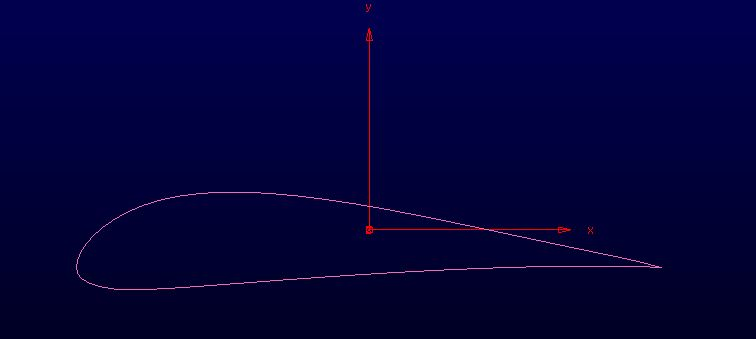
\includegraphics[width=\textwidth]{general_images/airfoil_image}
	\caption{Eppler 1210 Airfoil shown in Pointwise}
\label{fig:airfoil}
\end{figure}

\begin{table}[H]
\caption{Operating conditions for all cases}
	\centering
	\begin{tabular}{|r|r|} \hline
		Quantity & Value \\ \hline \hline
		Pressure & 101,325 Pa \\ \hline
		Temperature & 298 K  \\ \hline
		Velocity & 17.88 ms$^{-1}$ \\ \hline
		Viscosity & 1.789e-05 kgm$^{-1}$s$^{-1}$ \\ \hline
		Re \# & 1,224,315 \\ \hline
	\end{tabular}
\end{table}

\begin{table}[H]
\caption{XFoil Predictions, Re = 1e9, ncrit = 9 (clean wind tunnel)}
	\centering
	\begin{tabular}{|r|r|r|} \hline
				& Value	& AoA \\ \hline \hline
		Max L/D & 117.1309 & 8 \\ \hline
		Max $C_L$ & 1.8542 & 16 \\ \hline	
	\end{tabular}
\end{table}

% gradient: least squares cell based
% pressure: second order
% momentum: second order upwind
% turbulent kinetic energy: first order upwind
% specific dissipation rate: first order upwind
% intermittency: first order upwind
% momentum thickness Re: first order upwind

%\begin{figure}[h!]
%\centering
%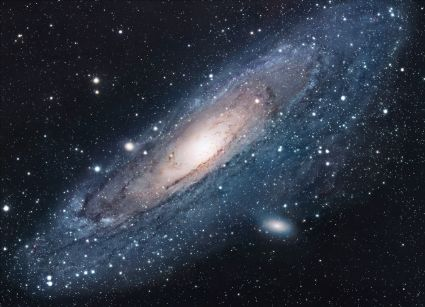
\includegraphics[scale=1.7]{universe}
%\caption{The Universe}
%\label{fig:universe}
%\end{figure}


\section{Methodology}

\begin{enumerate}
	\item 4 shots of grid: 1. LE 2. TE 3. near-field for entire shape 4. the entire grid domain. Note: should show T-rex feature that was used
	\item table 1: cell count and normal-to-wall spacing used, list BC, list reference values, list submodels chosen (i.e. viscous model), provide numerical scheme and spacial accuracy
	
\subsection{Screenshots of grid}

\begin{figure}[H]
	\centering
	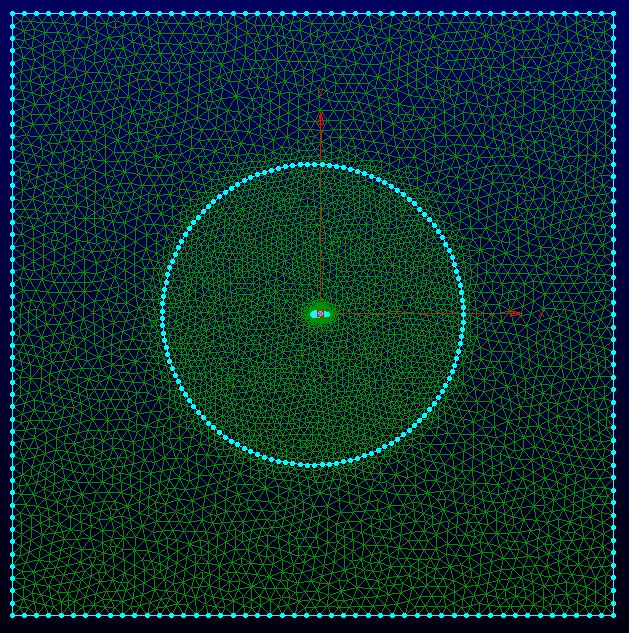
\includegraphics[width=\textwidth]{general_images/farfield}
	\caption{Farfield}
\label{fig:farfield}
\end{figure}

\begin{figure}[H]
	\centering
	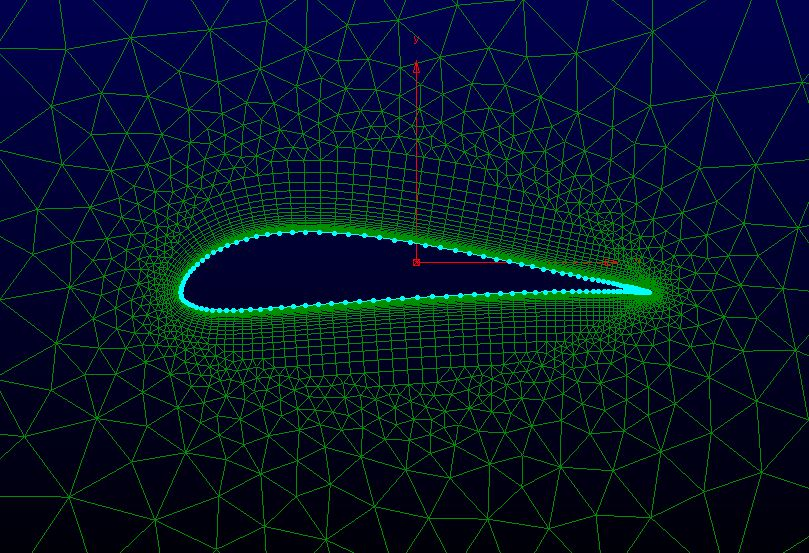
\includegraphics[width=0.9\textwidth]{general_images/nearfield}
	\caption{Nearfield}
\label{fig:nearfield}
\end{figure}	

\begin{figure}[H]
	\centering
	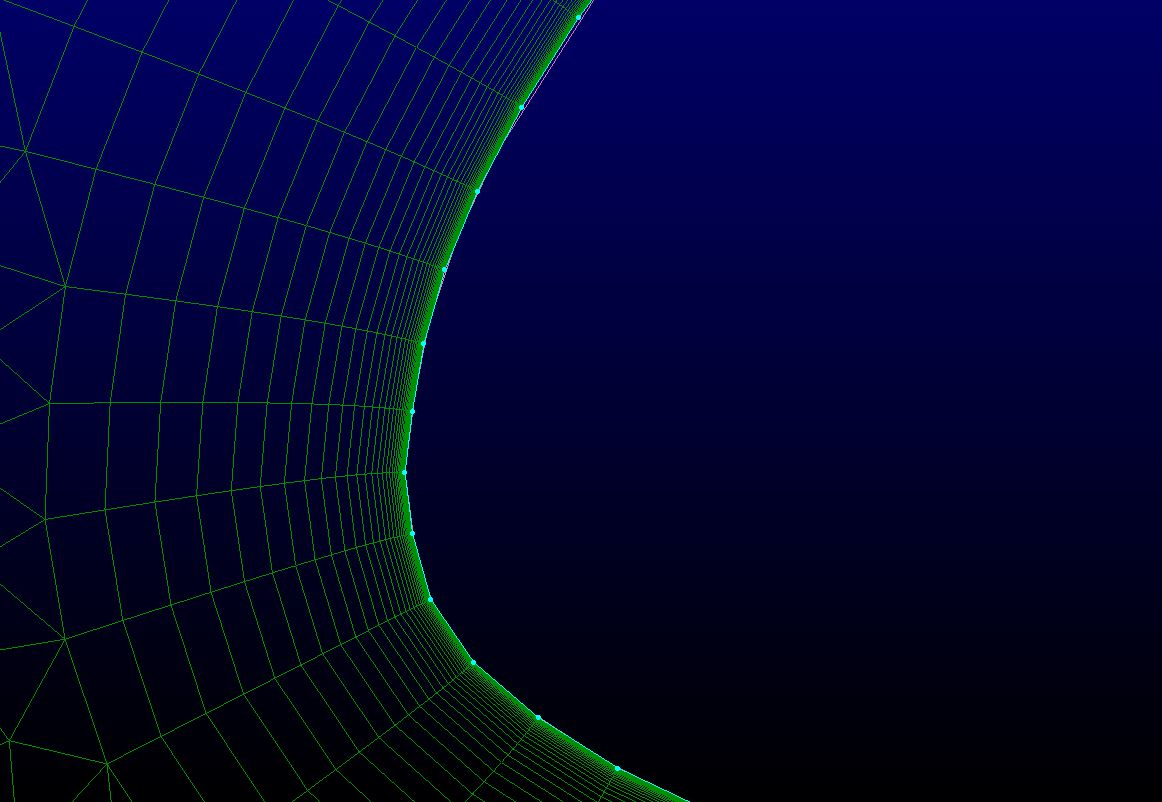
\includegraphics[width=0.9\textwidth]{general_images/LE1}
	\caption{Leading edge}
\label{fig:LE}
\end{figure}

\begin{figure}[H]
	\centering
	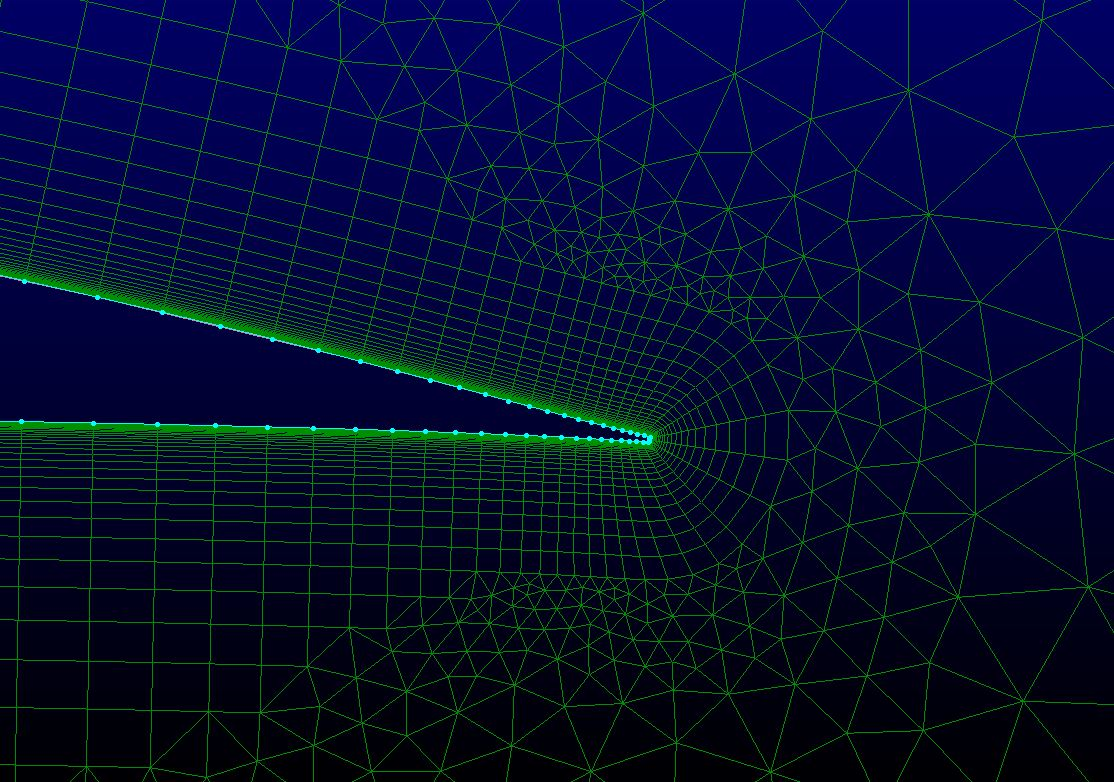
\includegraphics[width=0.9\textwidth]{general_images/TE1}
	\caption{Trailing edge}
\label{fig:TE}
\end{figure}

\begin{table}[H]
\caption{General grid information}
	\centering
	\begin{tabular}{|l|p{4.5in}|} \hline
				 & Value \\ \hline \hline
		Cell count & inner mesh: \newline outer mesh \\ \hline
		Normal-to-wall dist & 1e-5 (UNITS?) \\ \hline
		Boundary condition & airfoil surface: wall, $\Delta$s=1e-5 \newline (might have to specify at inlet and such, check) \\ \hline
		Reference values & A bunch of different ones here, 1.789e-05 kgm$^{-1}$s$^{-1}$ \\ \hline
		Submodels & viscous: transitional SST \\ \hline
		Numerical Schemes & \textbf{gradient}: least-squares cell based \newline \textbf{pressure}: second order \newline \textbf{momentum}: second order upwind \newline \textbf{turbulent kinetic energy}: first order upwind \newline \textbf{specific dissipation rate}: first order upwind \newline \textbf{specific dissipation rate}: first order upwind \newline \textbf{intermittency}: first order upwind \newline \textbf{momentum thickness Re}: first order upwind \\ \hline
	\end{tabular}
\end{table}



% gradient: least squares cell based
% pressure: second order
% momentum: second order upwind
% turbulent kinetic energy: first order upwind
% specific dissipation rate: first order upwind
% intermittency: first order upwind
% momentum thickness Re: first order upwind
		
\end{enumerate}

\section{Results}

\begin{enumerate}
	\item plot lift and drag coeff histories for proof of convergence history for ALL Runs (appendix)
	\item Table of $C_l$, $C_d$, L/D, $C_m$
	\item plots of the items in the table and compared against Xfoil data at the closest Re \# (take directly from airfoiltools.com)
	\item streamlines and pressure contours to depict flow near airfoil
	\begin{itemize}
		\item 1 plot for each case
		\item use the same contour levels
	\end{itemize}
	\item y+ curves (for $0^\circ$ AoA case)
	\item plot showing turbulent boundary layer development ($0^\circ$ AoA case)
\end{enumerate}

\subsection{Plots of convergence history for all runs}
See Appendix A

\subsection{Table of final force/moment coefficient values}

\begin{table}[H]
\caption{Some aerodynamic coefficients}
\centering
\begin{tabular}{|l|l|l|l|l|} \hline
\textbf{AoA ($^\circ$)} & $\boldsymbol{C_l}$ & $\boldsymbol{C_d}$ & $\boldsymbol{C_m}$ & \textbf{L/D} \\ \hline \hline
-7           & -0.2475        & 0.0129         & -0.0317        & -19.1200     \\ \hline
-4           & 0.0771         & 0.0106         & -0.1102        & 7.3024       \\ \hline
-2           & 0.1864         & 0.0105         & -0.1368        & 17.7983      \\ \hline
0            & 0.5159         & 0.0106         & -0.0891        & 48.5390      \\ \hline
5            & 1.0736         & 0.0119         & -0.3562        & 90.3674      \\ \hline
8.5          & 1.4360         & 0.0173         & -0.4419        & 82.7872      \\ \hline
12           & 1.7358         & 0.0261         & -0.5071        & 66.4839      \\ \hline
14.5         & 1.8475         & 0.0381         & -0.5246        & 48.5187      \\ \hline
17           & 1.6456         & 0.0890         & -0.4857        & 18.4886      \\ \hline
19.5         & 1.3897         & 0.1635         & -0.4471        & 8.4988       \\ \hline
22           & 1.2712         & 0.2341         & -0.4433        & 5.4310       \\ \hline
\end{tabular}
\end{table}

\begin{figure}[H]
	\centering
	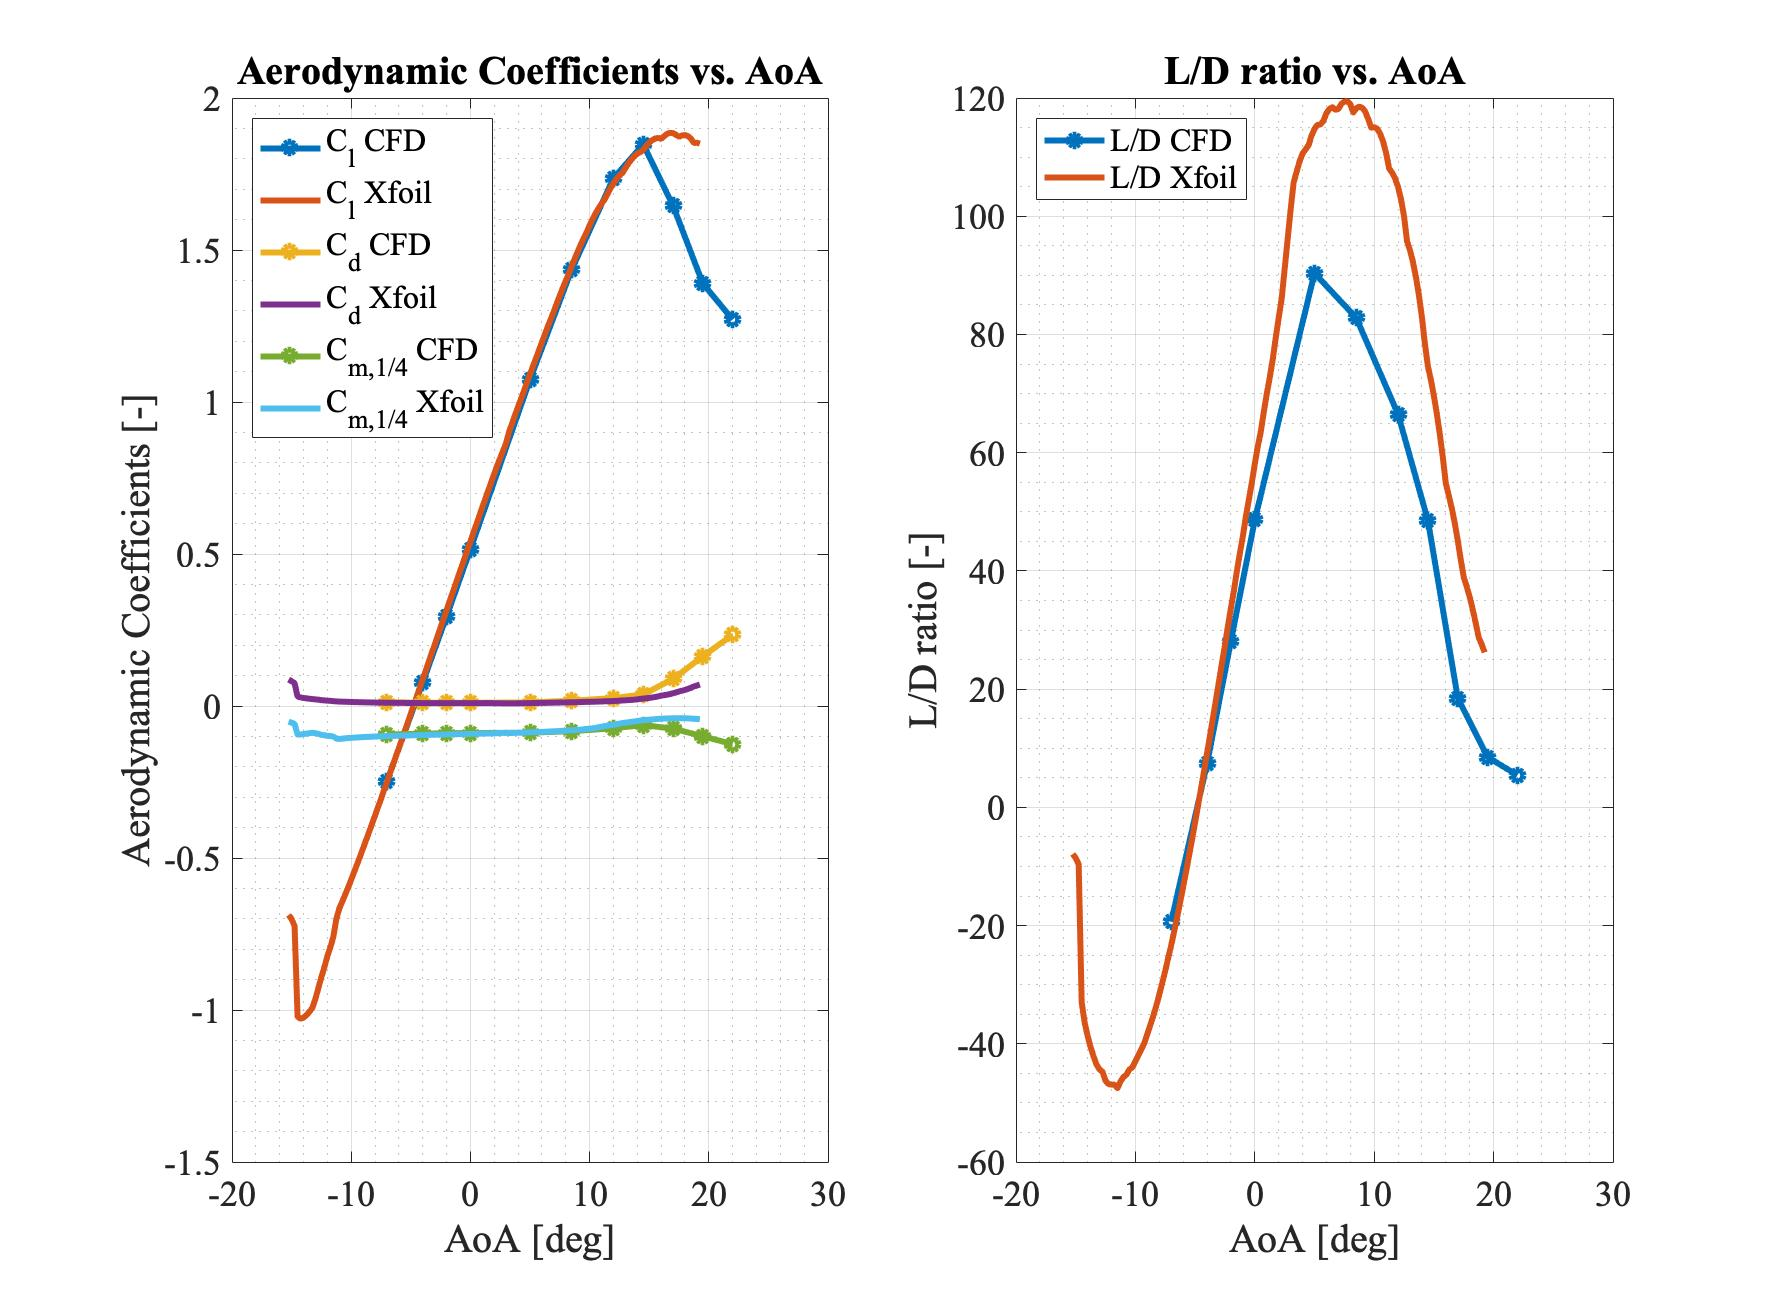
\includegraphics[width=\textwidth]{coeffs.jpg}
	\caption{Comparison of aerodynamic coefficients from Xfoil and CFD}
\label{fig:coeffs}
\end{figure}

\subsection{Pressure contours and streamlines}

\begin{figure}[H]
	\centering
	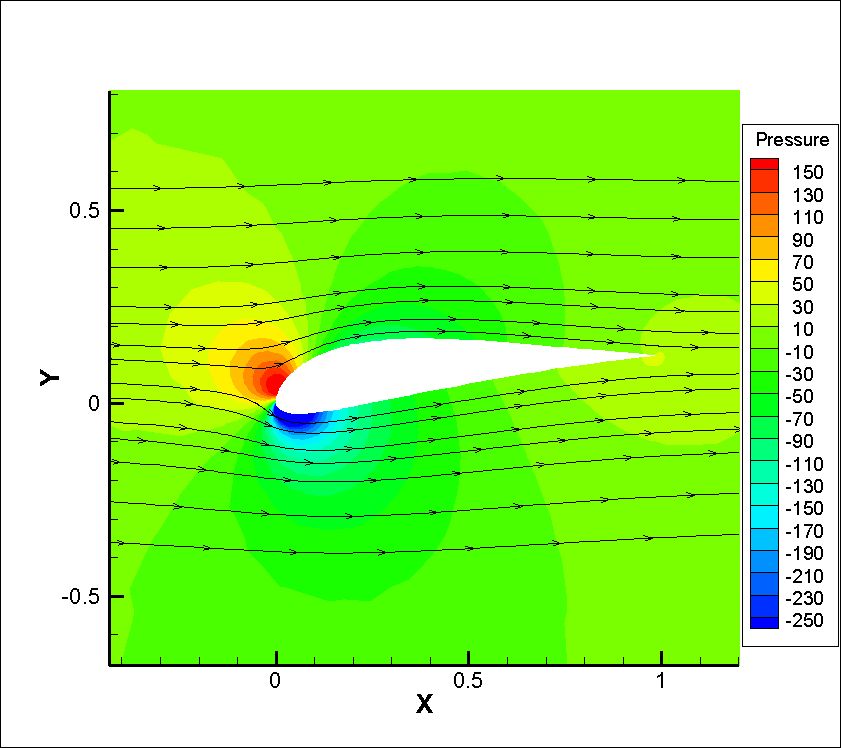
\includegraphics[width=0.6\textwidth]{tecplot_stuff/cont_stream_-7.png}
	\caption{Pressure contours and streamlines for AoA = -7$^\circ$}
\label{fig:cont_stream_-7}
\end{figure}

\begin{figure}[H]
	\centering
	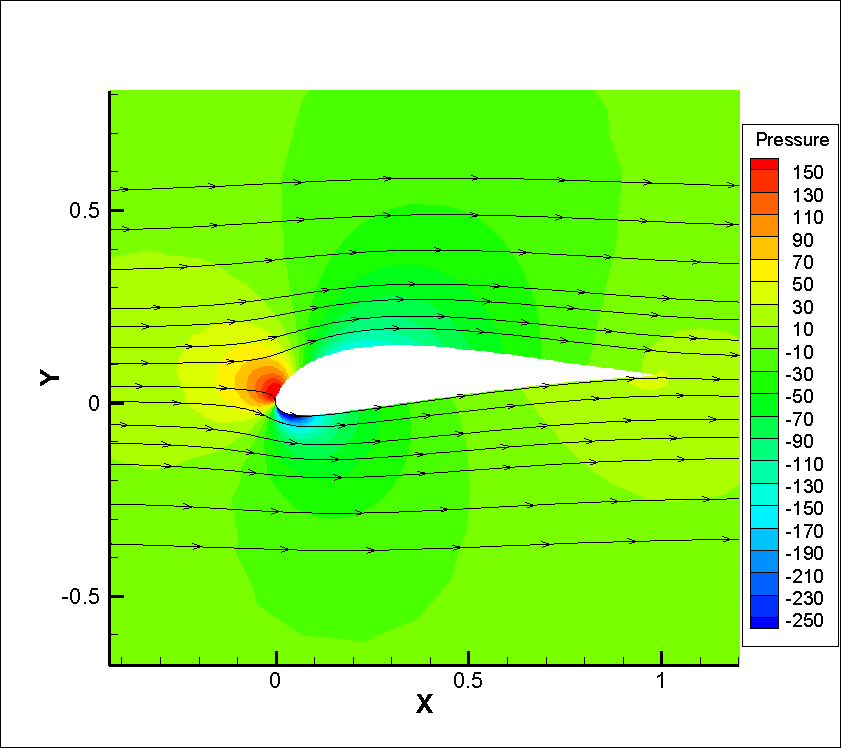
\includegraphics[width=0.6\textwidth]{tecplot_stuff/cont_stream_-4.png}
	\caption{Pressure contours and streamlines for AoA = -4$^\circ$}
\label{fig:cont_stream_-4}
\end{figure}


\begin{figure}[H]
	\centering
	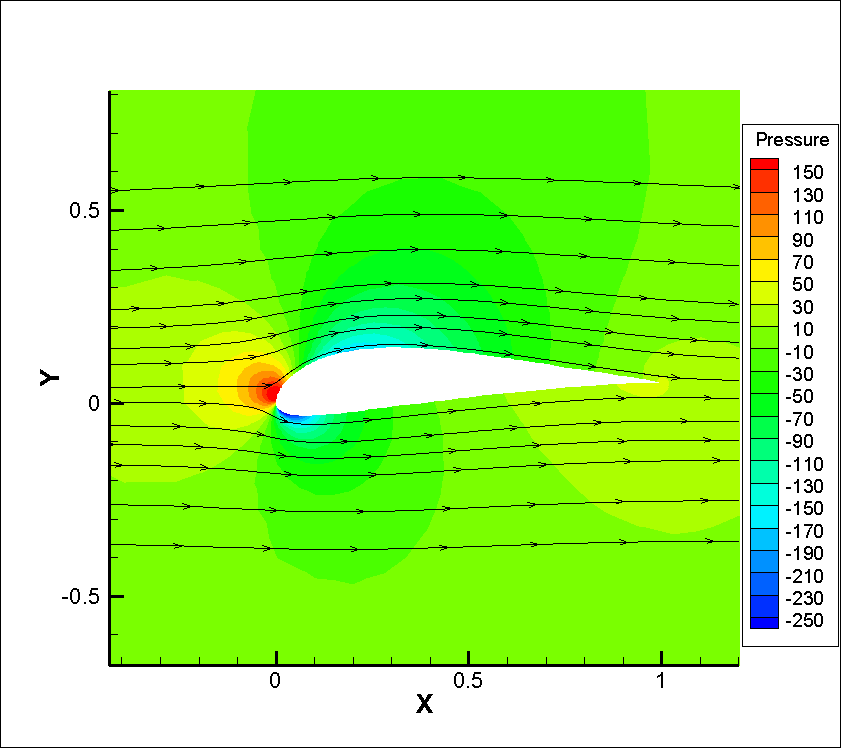
\includegraphics[width=0.6\textwidth]{tecplot_stuff/cont_stream_-2.png}
	\caption{Pressure contours and streamlines for AoA = -2$^\circ$}
\label{fig:cont_stream_-2}
\end{figure}


\begin{figure}[H]
	\centering
	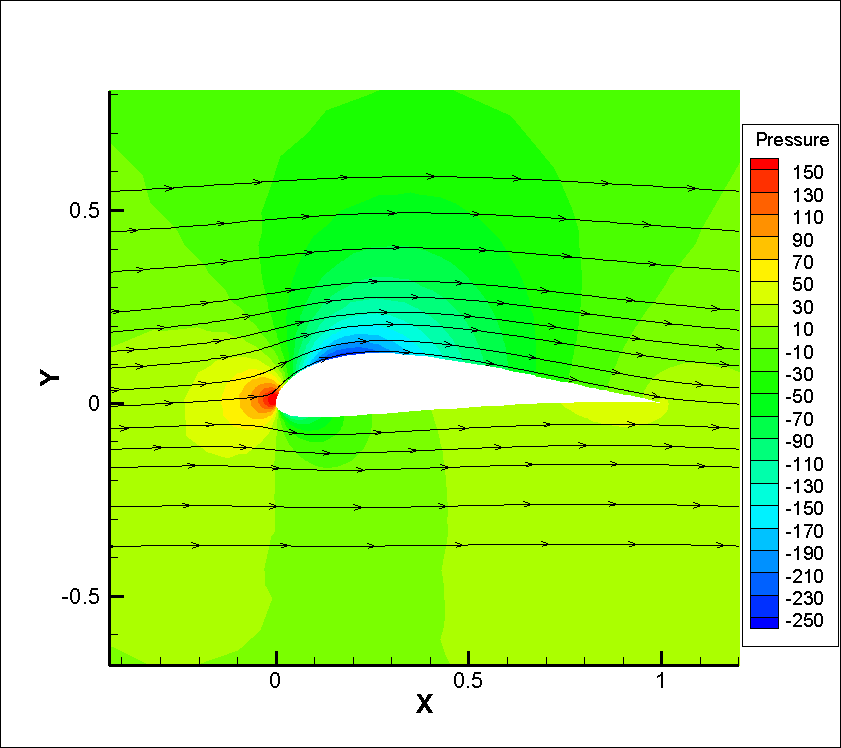
\includegraphics[width=0.6\textwidth]{tecplot_stuff/cont_stream_0.png}
	\caption{Pressure contours and streamlines for AoA = 0$^\circ$}
\label{fig:cont_stream_0}
\end{figure}


\begin{figure}[H]
	\centering
	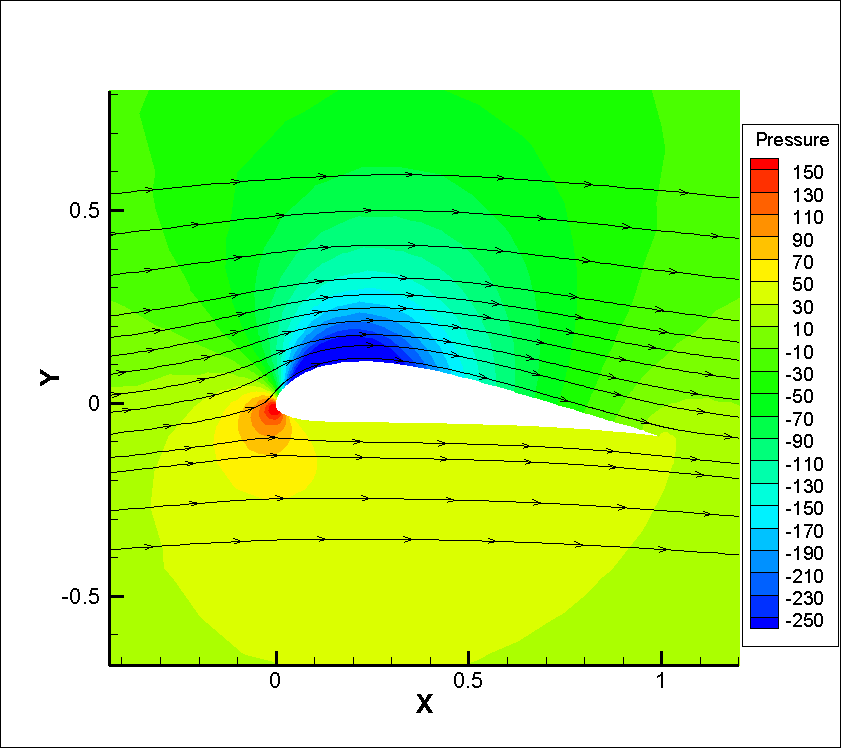
\includegraphics[width=0.6\textwidth]{tecplot_stuff/cont_stream_5.png}
	\caption{Pressure contours and streamlines for AoA = 5$^\circ$}
\label{fig:cont_stream_5}
\end{figure}


\begin{figure}[H]
	\centering
	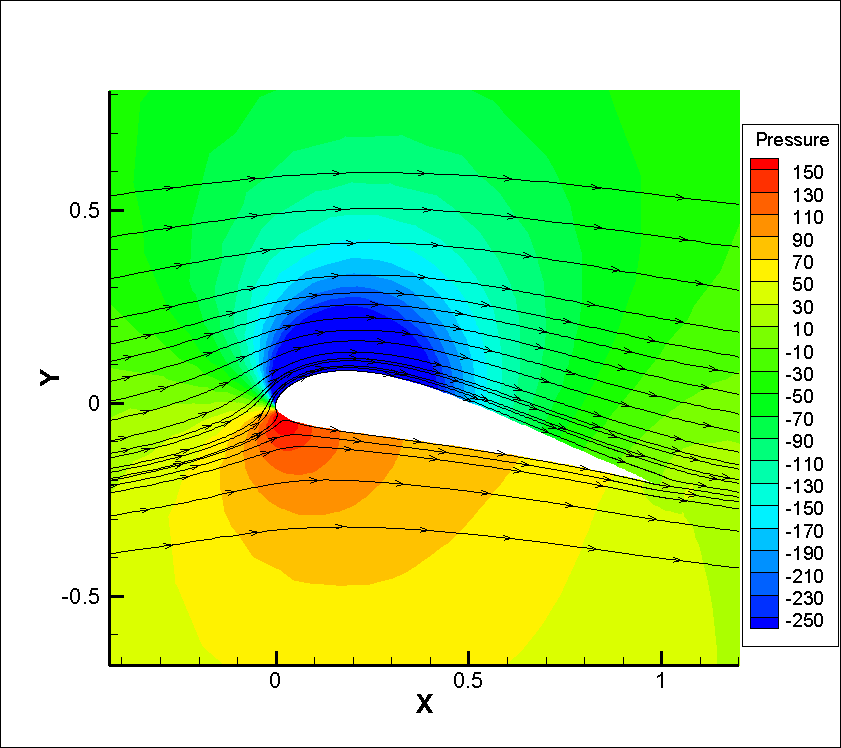
\includegraphics[width=0.6\textwidth]{tecplot_stuff/cont_stream_12.png}
	\caption{Pressure contours and streamlines for AoA = 12$^\circ$}
\label{fig:cont_stream_12}
\end{figure}

\begin{figure}[H]
	\centering
	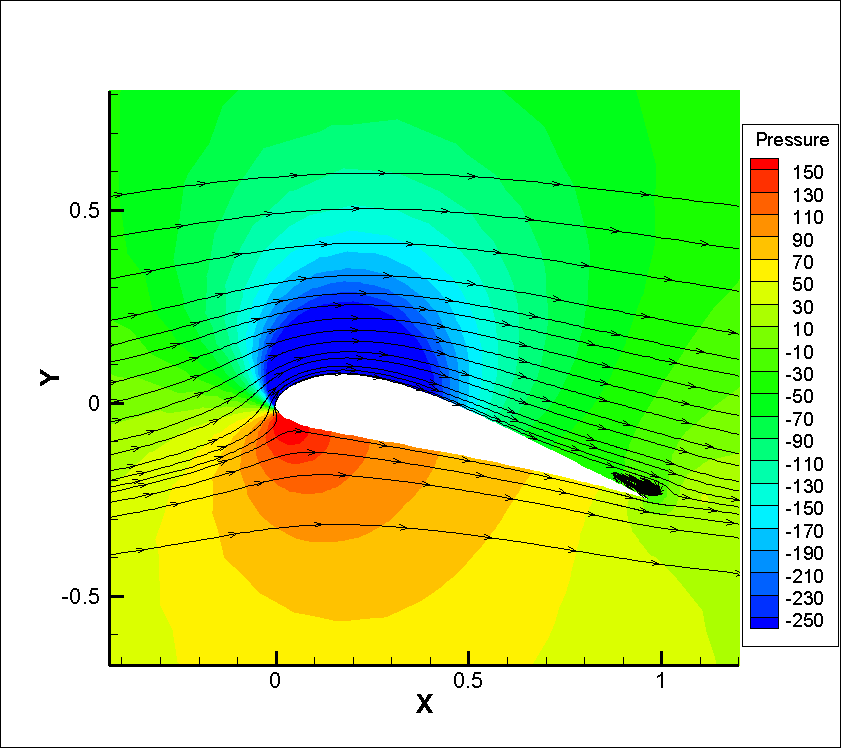
\includegraphics[width=0.6\textwidth]{tecplot_stuff/cont_stream_14_5.png}
	\caption{Pressure contours and streamlines for AoA = 14.5$^\circ$}
\label{fig:cont_stream_14_5}
\end{figure}

\begin{figure}[H]
	\centering
	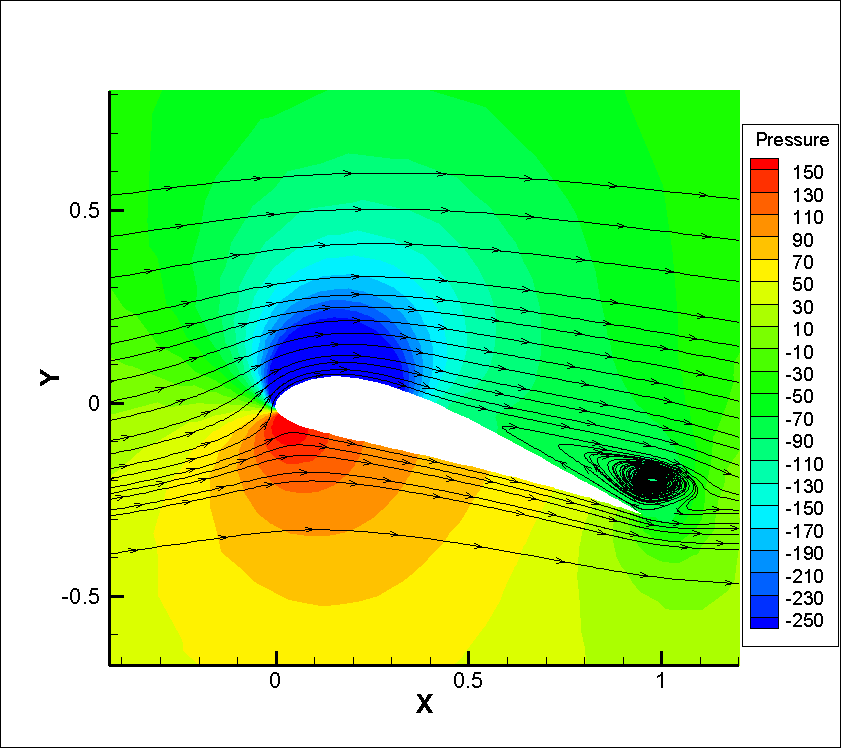
\includegraphics[width=0.6\textwidth]{tecplot_stuff/cont_stream_17.png}
	\caption{Pressure contours and streamlines for AoA = 17$^\circ$}
\label{fig:cont_stream_17}
\end{figure}

\begin{figure}[H]
	\centering
	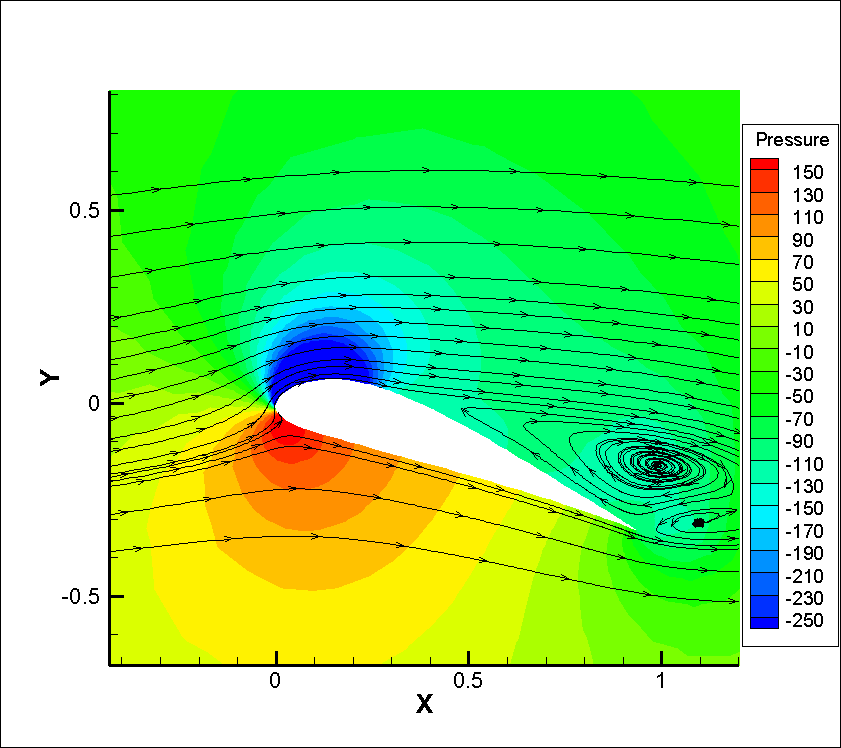
\includegraphics[width=0.6\textwidth]{tecplot_stuff/cont_stream_19_5.png}
	\caption{Pressure contours and streamlines for AoA = 19.5$^\circ$}
\label{fig:cont_stream_19_5}
\end{figure}

\begin{figure}[H]
	\centering
	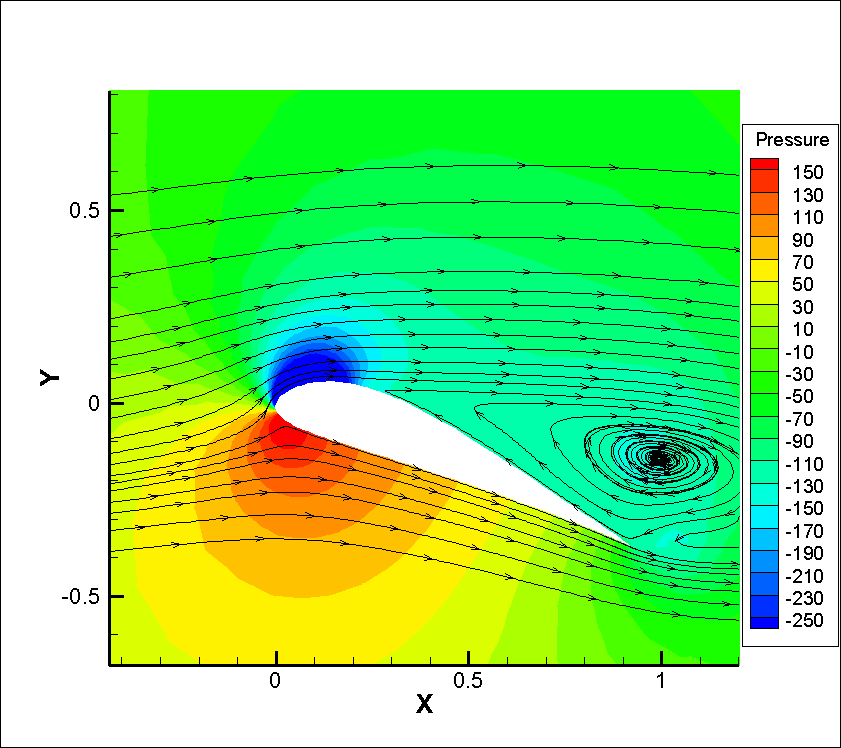
\includegraphics[width=0.6\textwidth]{tecplot_stuff/cont_stream_22.png}
	\caption{Pressure contours and streamlines for AoA = 22$^\circ$}
\label{fig:cont_stream_22}
\end{figure}

\subsection{y+ Curve}

\begin{figure}[H]
	\centering
	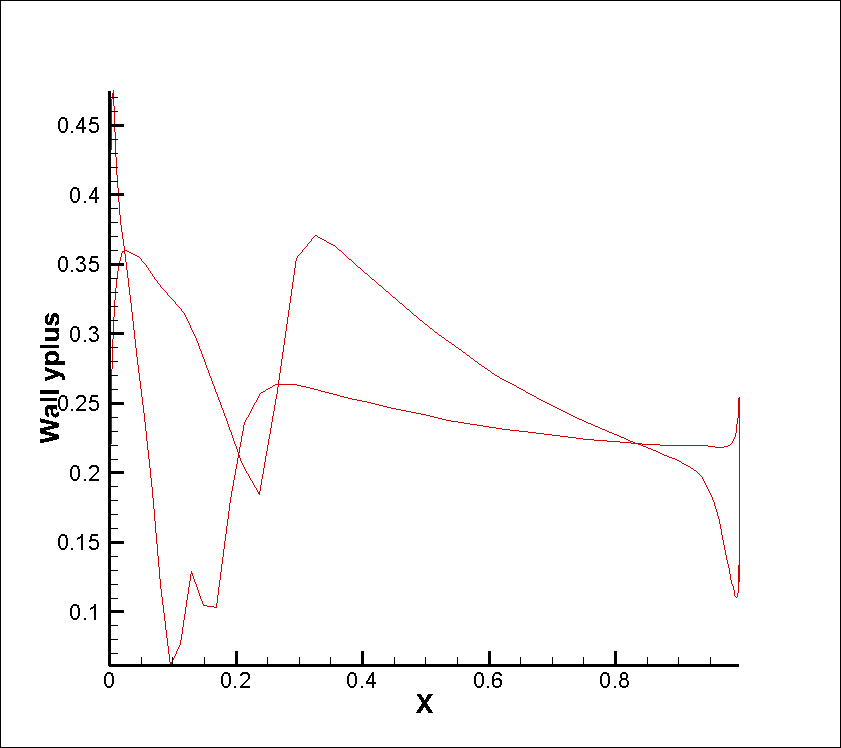
\includegraphics[width=0.6\textwidth]{tecplot_stuff/y_plus_0.png}
	\caption{y plus graph}
\label{fig:yplus}
\end{figure}

\subsection{Turbulent Boundary Layer Development}

\begin{figure}[H]
	\centering
	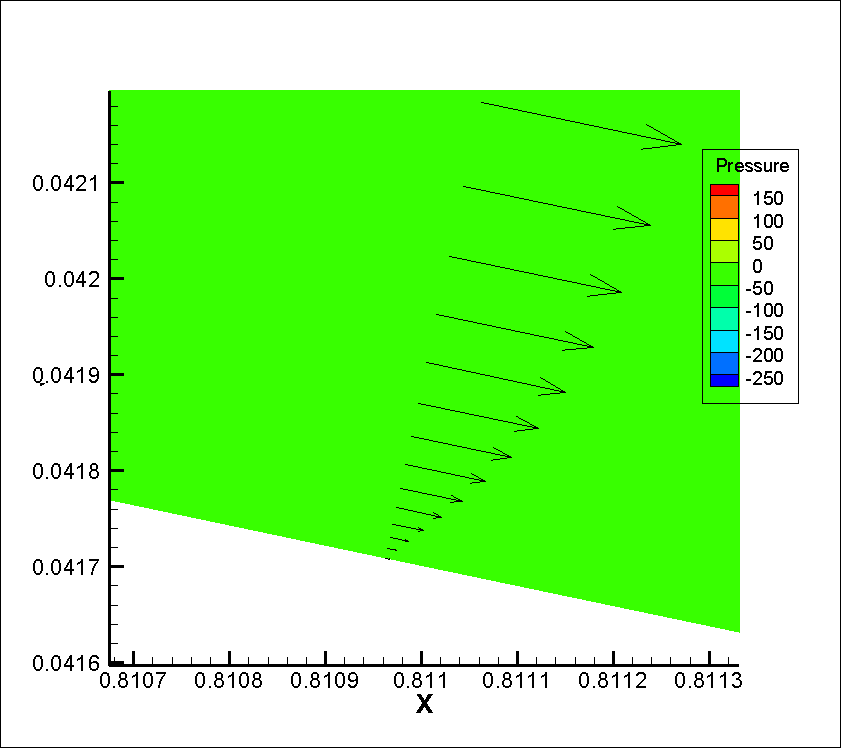
\includegraphics[width=0.6\textwidth]{tecplot_stuff/BL_0.png}
	\caption{Boundary layer near trailing edge of wing}
\label{fig:BL}
\end{figure}


\section{Discussion}

Taking the XFoil data as "experimental," and the CFD data as numerical prediction, error bars of $\pm10\%$ were drawn from each XFoil data point. Observing the $C_l$ first in Fig. \ref{fig:error_bar1}, XFoil and CFD agree very well until separation, where CFD predict its happening at a lower AoA. In this case, the CFD simulation might be more trustworthy, as it is difficult to predict separation, especially with low-fidelity methods. Regarding $C_d$, the CFD generally overpredicted the XFoil solution as seen in Figs. \ref{fig:error_bar2} and \ref{fig:error_bar3}, zoomed-in view of the exact same same figure. The former is at small negative AoAs, where the CFD prediction is about 10\% above XFoil prediction; this was as close as the two solutions ever came. Higher AoAs led to larger discrepancies, where the CFD predictions increasingly overpredicted the XFoil estimates. This discrepancy can be attributed to numerical diffusion created by second order schemes?

\begin{figure}[H]
\centering
    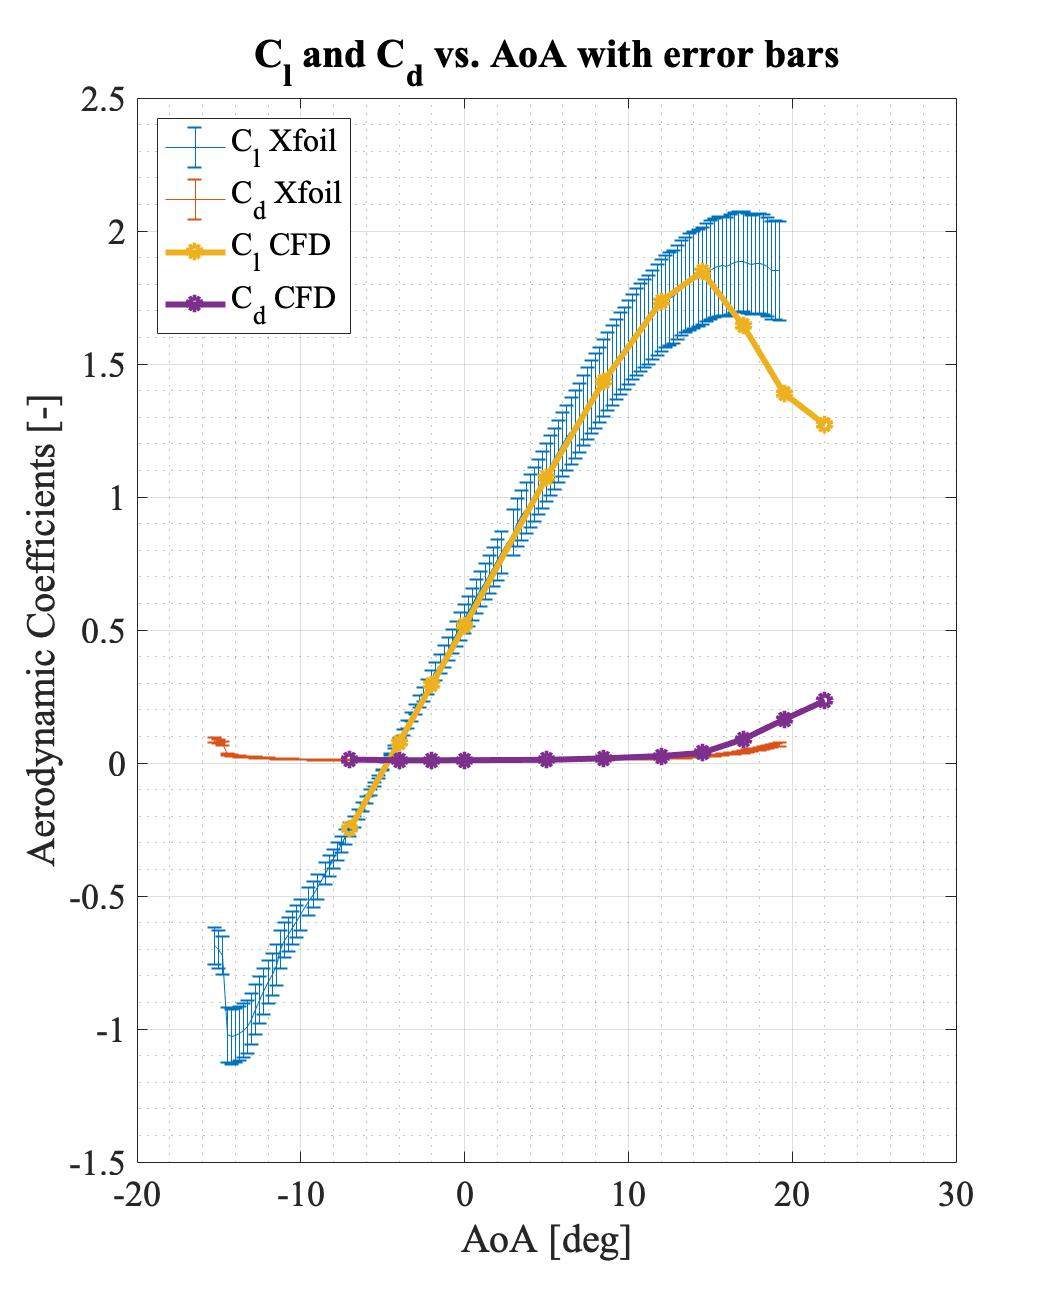
\includegraphics[width=0.65\textwidth]{error_bar1.jpg}
    \caption{$C_l$ and $C_d$ comparisons including error bar of $\pm$10\%}
    \label{fig:error_bar1}
\end{figure}

\begin{figure}[H]
  \begin{subfigure}[b]{0.5\textwidth}
    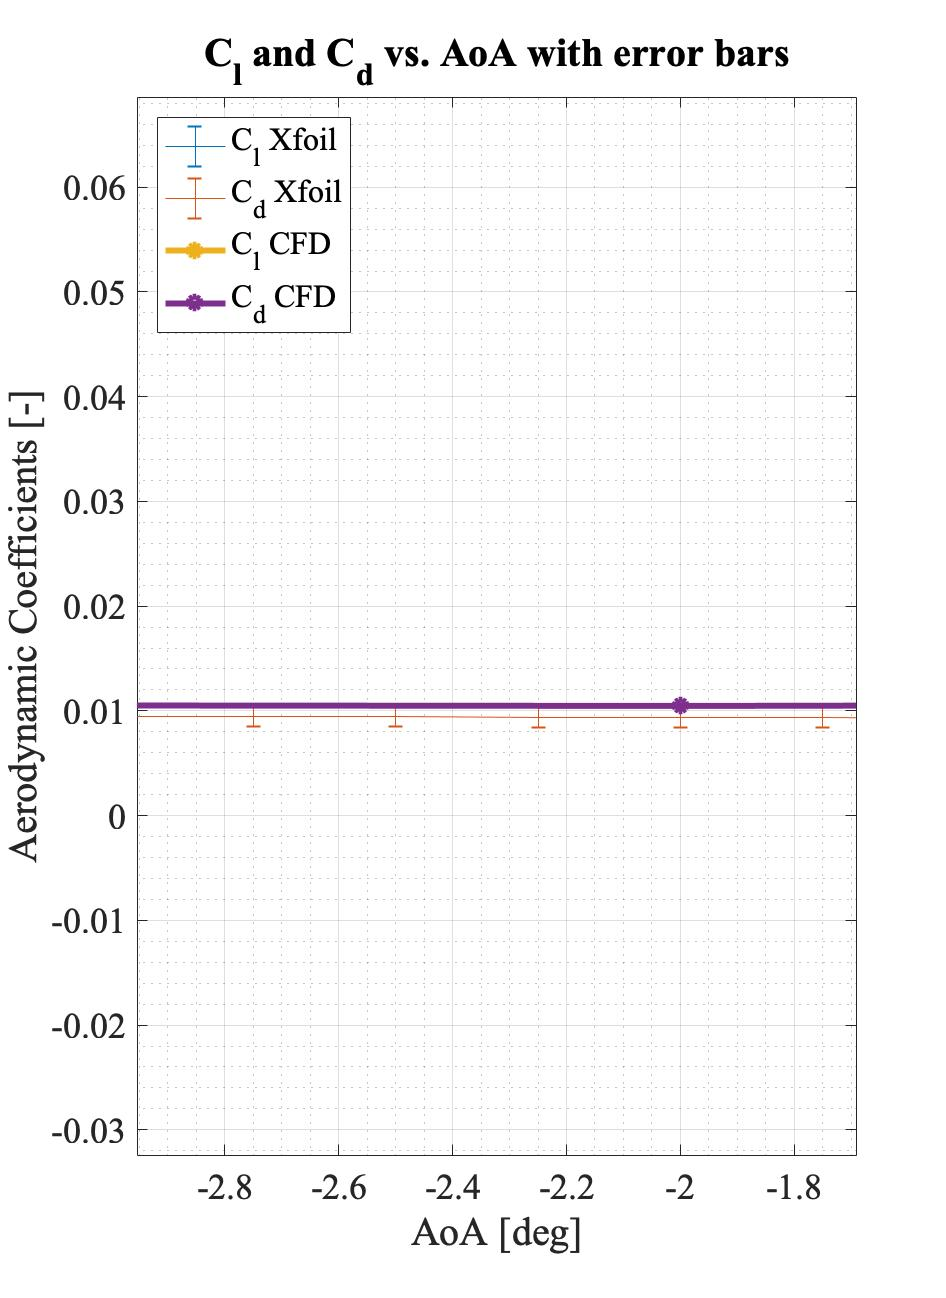
\includegraphics[width=\textwidth]{error_bar2.jpg}
    \caption{Zoomed-in view of lower AoA section of $C_d$}
    \label{fig:error_bar2}
  \end{subfigure}
  \begin{subfigure}[b]{0.5\textwidth}
    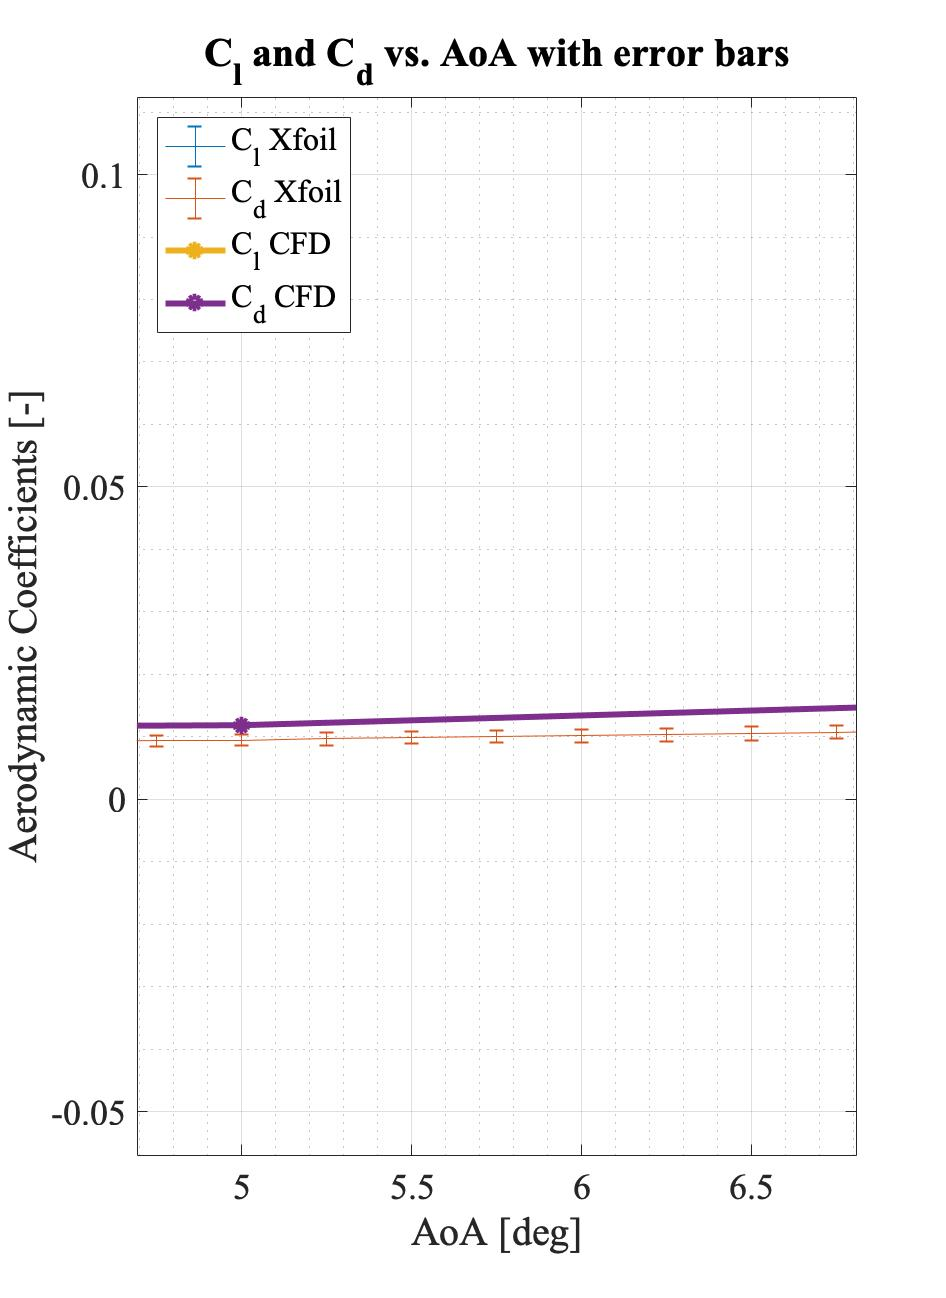
\includegraphics[width=\textwidth]{error_bar3.jpg}
    \caption{Another zoomed-in view of larger AoA section of $C_d$}
    \label{fig:error_bar3}
  \end{subfigure}
\end{figure}


\section*{Appendix A}

\subsection*{AoA = -7$^\circ$}

%\begin{figure}[!tbp]
%  \centering
%  \begin{minipage}[b]{0.45\textwidth}
%    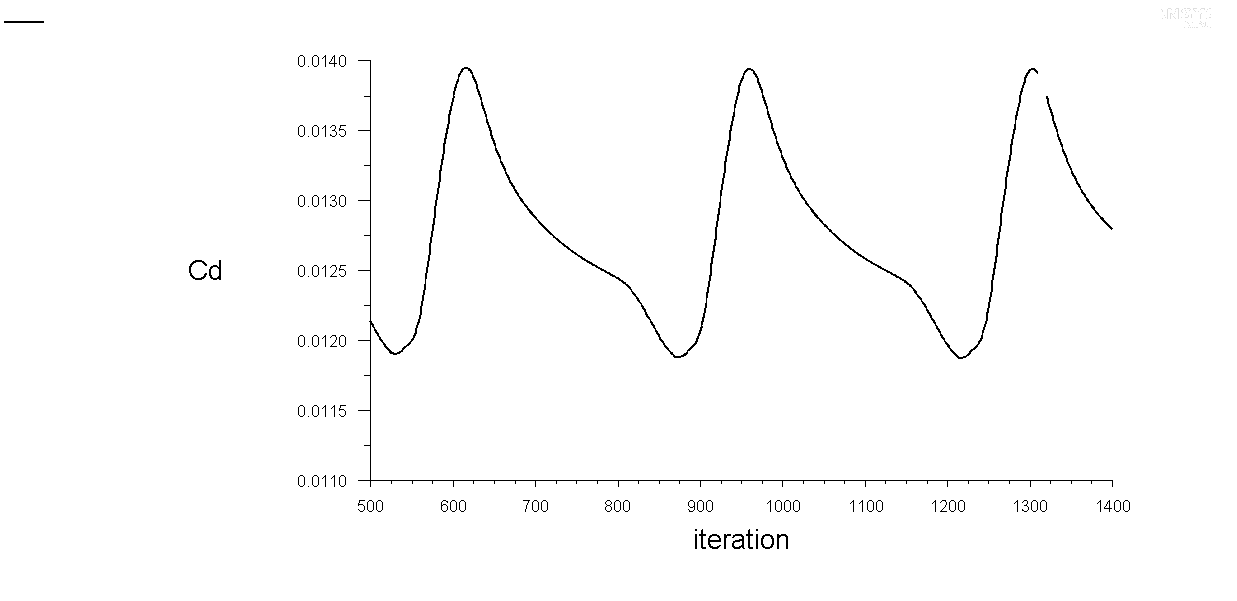
\includegraphics[width=\textwidth]{-7_deg/AoA_-7_cd}
%    \caption{Flower one.}
%  \end{minipage}
%  \hfill
%  \begin{minipage}[b]{0.4\textwidth}
%    \includegraphics[width=\textwidth]{flower2.jpg}
%    \caption{Flower two.}
%  \end{minipage}
%\end{figure}

% ************************ -7 degs ****************************

\begin{figure}[H]
  \begin{subfigure}[b]{0.5\textwidth}
    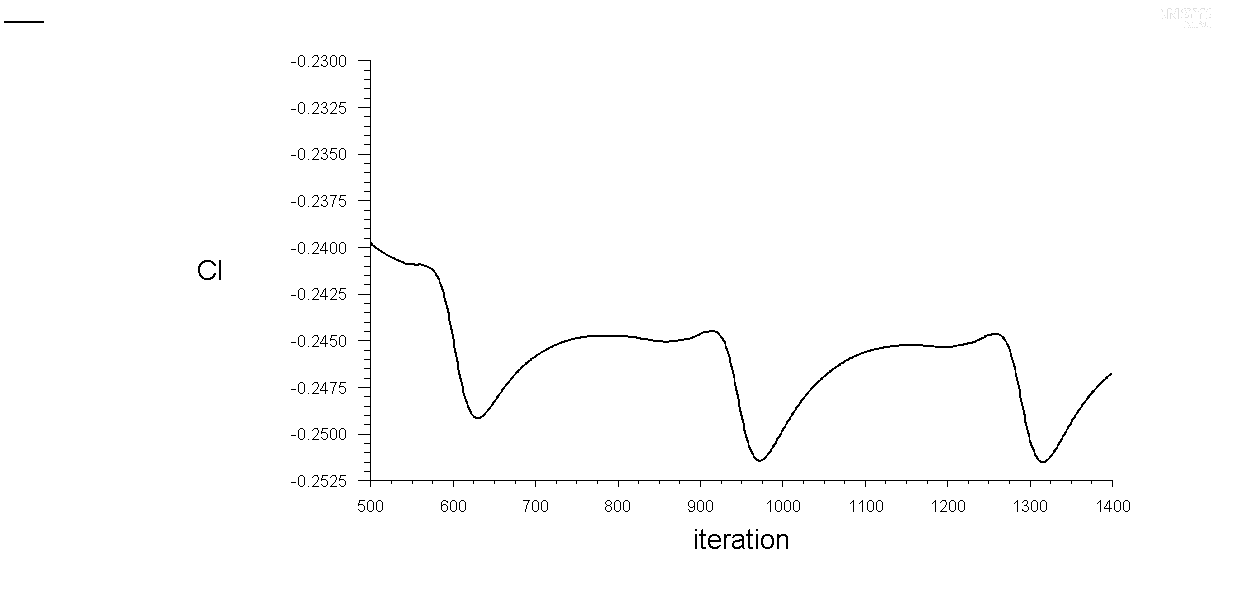
\includegraphics[width=\textwidth]{-7_deg/AoA_-7_cl.png}
    \caption{$C_l$ for AoA = -7$^\circ$}
    \label{fig:aoa_-7_cl}
  \end{subfigure}
  \hfill
  \begin{subfigure}[b]{0.5\textwidth}
    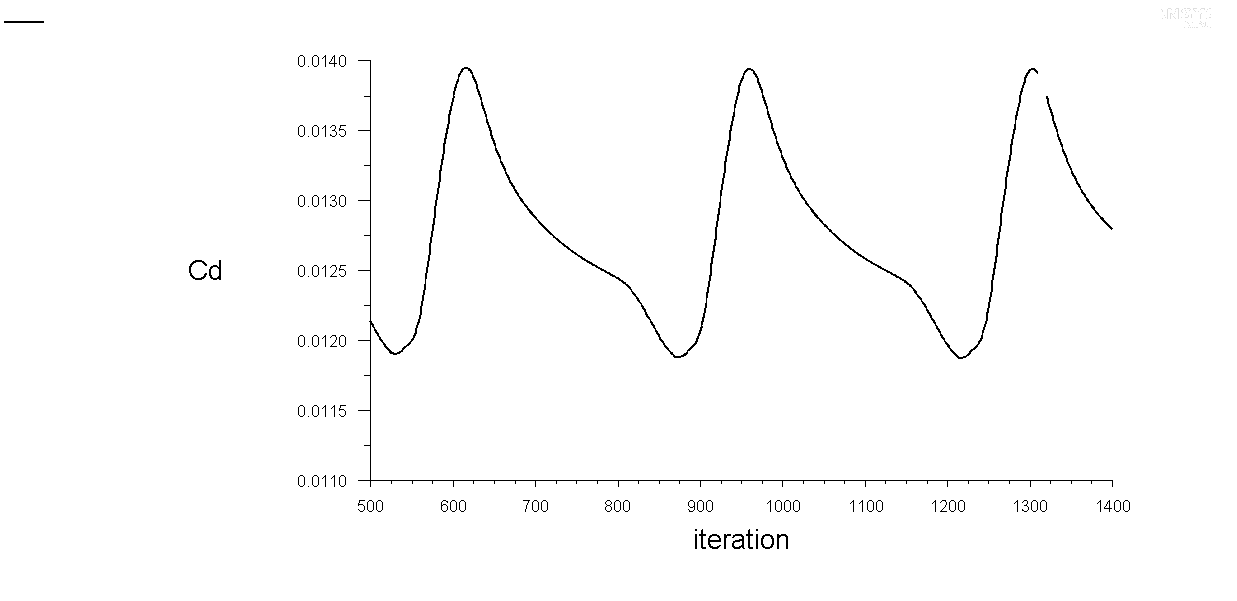
\includegraphics[width=\textwidth]{-7_deg/AoA_-7_cd.png}
    \caption{$C_d$ for AoA = -7$^\circ$}
    \label{fig:aoa_-7_cd}
  \end{subfigure}
  \begin{subfigure}[b]{0.5\textwidth}
    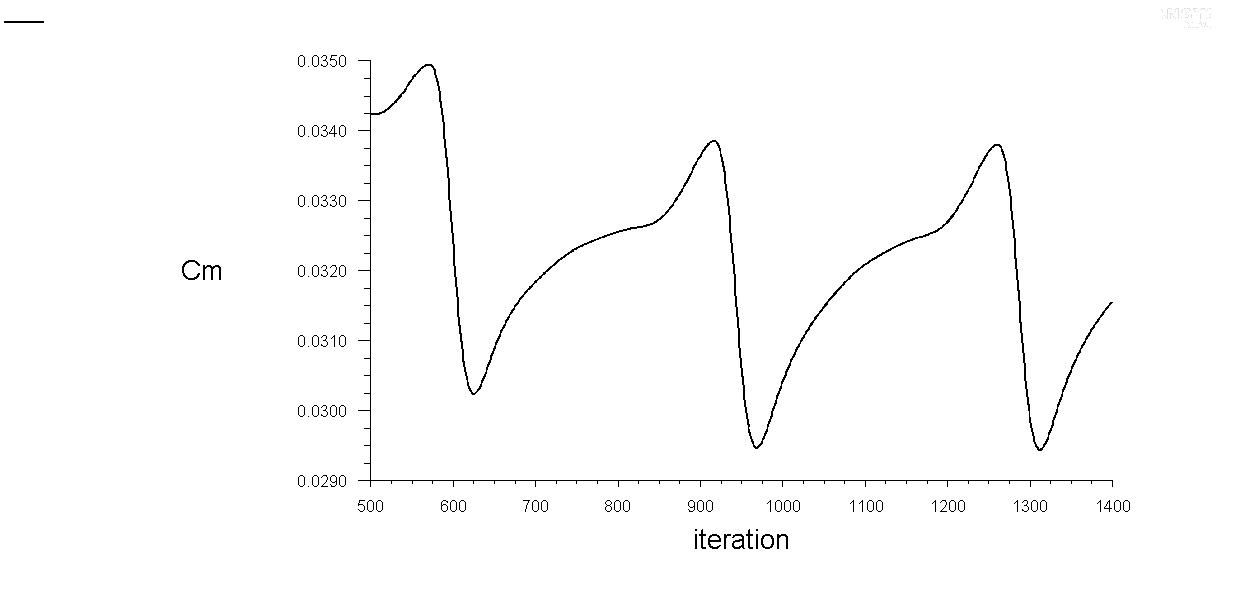
\includegraphics[width=\textwidth]{-7_deg/AoA_-7_cm.png}
    \caption{$C_m$ for AoA = -7$^\circ$}
    \label{fig:aoa_-7_cm}
  \end{subfigure}
  \begin{subfigure}[b]{0.5\textwidth}
    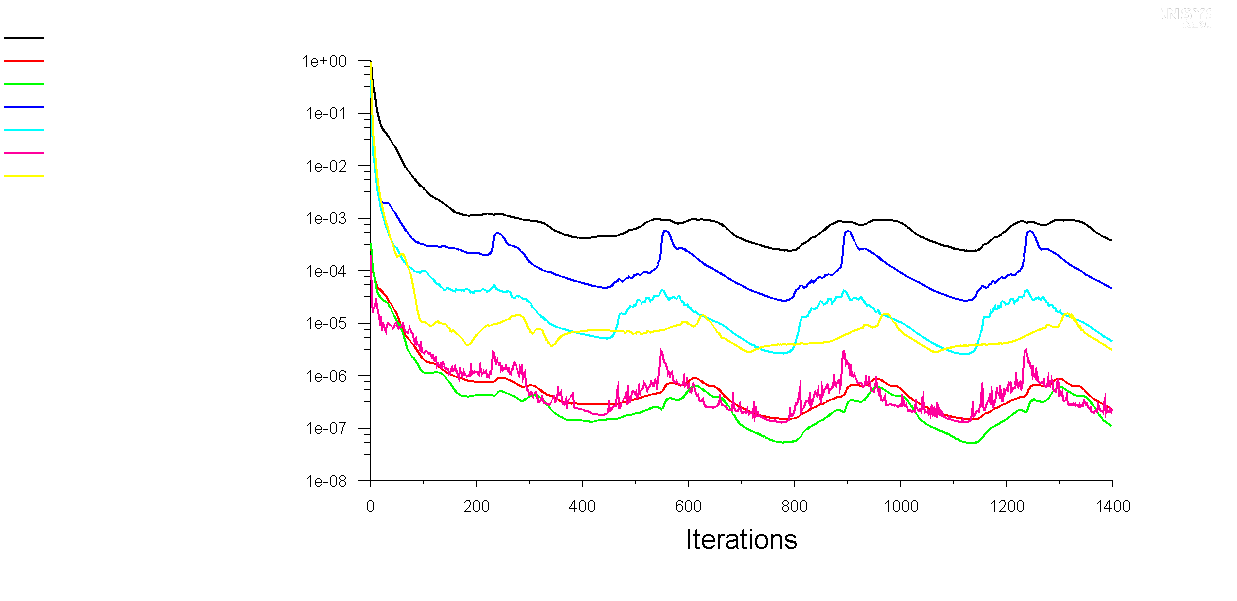
\includegraphics[width=\textwidth]{-7_deg/AoA_-7_resid.png}
    \caption{Residual plot for AoA = -7$^\circ$}
    \label{fig:aoa_-7_resid}
  \end{subfigure}
\end{figure}


% ************************ -4 degs ****************************
\subsection*{AoA = -4$^\circ$}

\begin{figure}[H]
  \begin{subfigure}[b]{0.5\textwidth}
    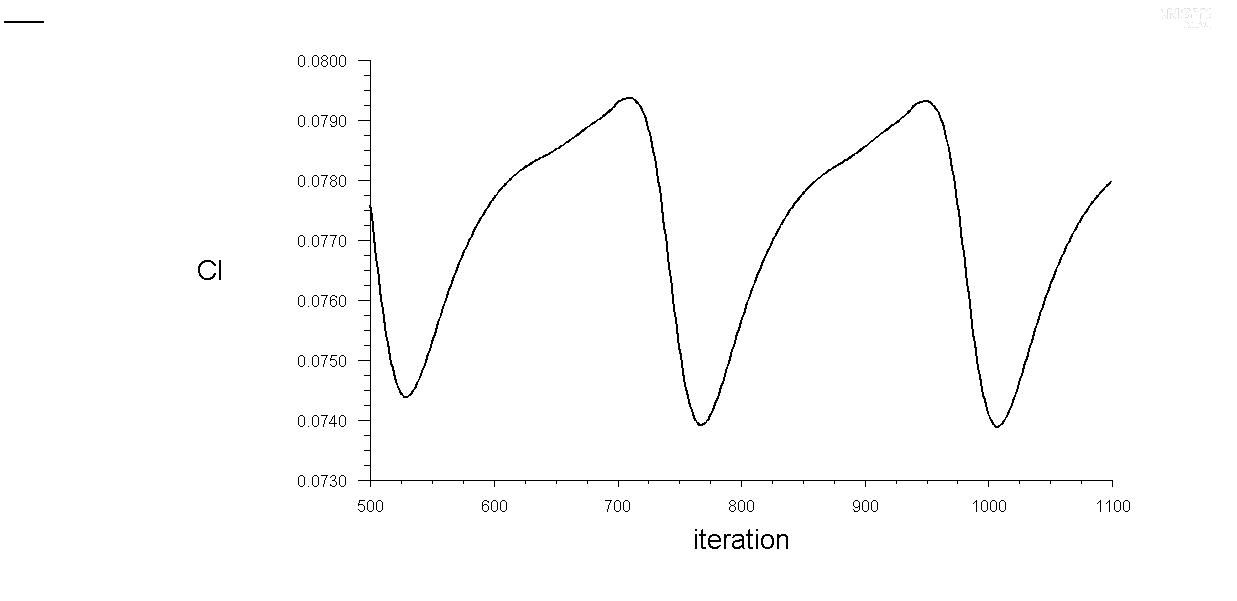
\includegraphics[width=\textwidth]{-4_deg/AoA_-4_cl.png}
    \caption{$C_l$ for AoA = -4$^\circ$}
    \label{fig:aoa_-4_cl}
  \end{subfigure}
  \hfill
  \begin{subfigure}[b]{0.5\textwidth}
    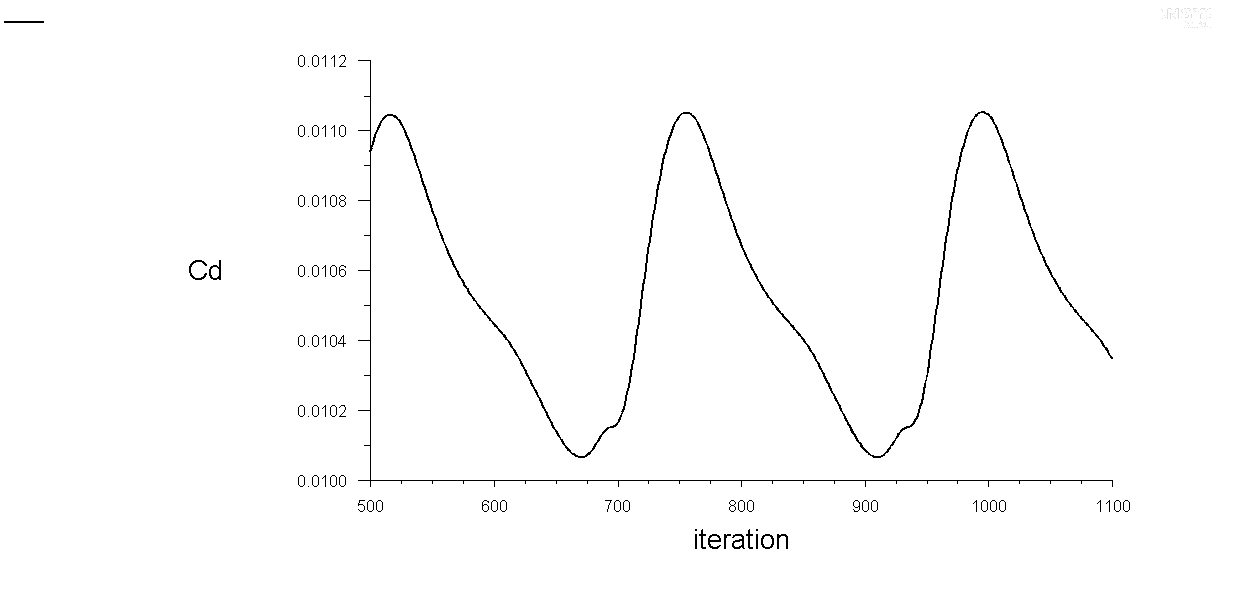
\includegraphics[width=\textwidth]{-4_deg/AoA_-4_cd.png}
    \caption{$C_d$ for AoA = -4$^\circ$}
    \label{fig:aoa_-4_cd}
  \end{subfigure}
  \begin{subfigure}[b]{0.5\textwidth}
    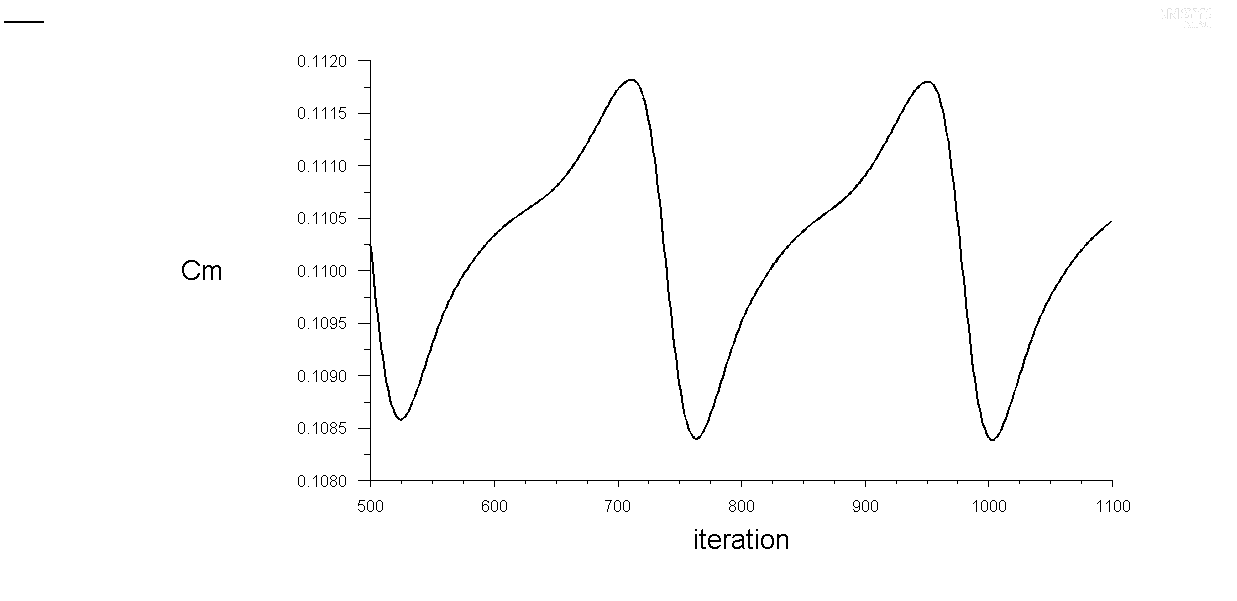
\includegraphics[width=\textwidth]{-4_deg/AoA_-4_cm.png}
    \caption{$C_m$ for AoA = -4$^\circ$}
    \label{fig:aoa_-4_cm}
  \end{subfigure}
  \begin{subfigure}[b]{0.5\textwidth}
    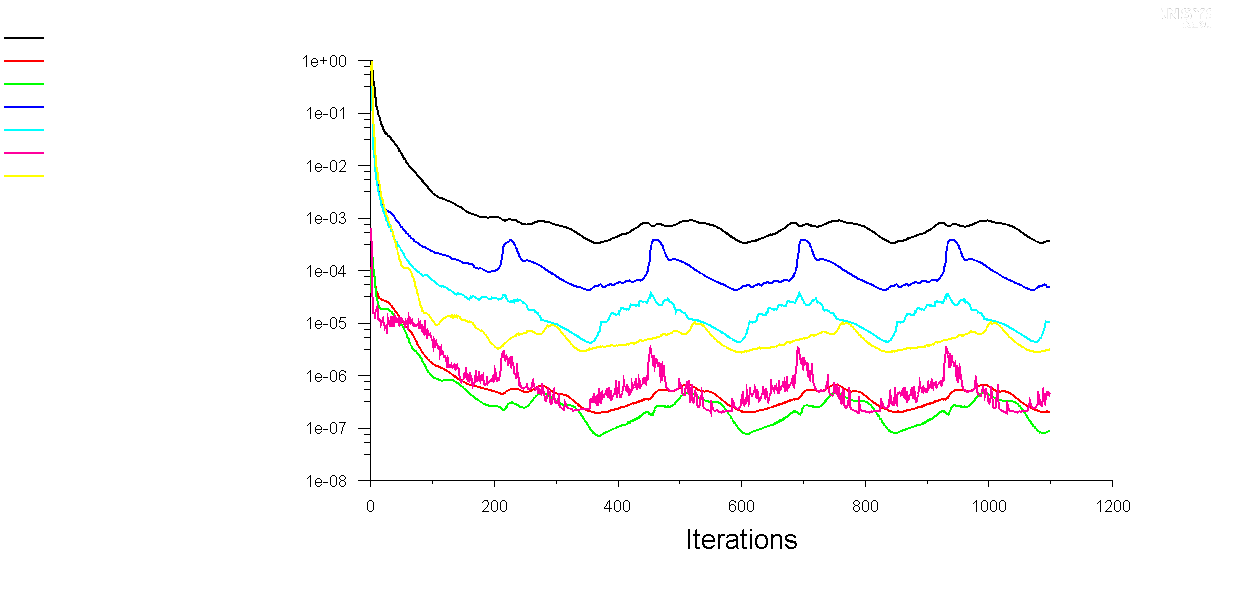
\includegraphics[width=\textwidth]{-4_deg/AoA_-4_resid.png}
    \caption{Residual plot for AoA = -4$^\circ$}
    \label{fig:aoa_-4_resid}
  \end{subfigure}
\end{figure}

% ************************ -2 degs ****************************
\subsection*{AoA = -2$^\circ$}

\begin{figure}[H]
  \begin{subfigure}[b]{0.5\textwidth}
    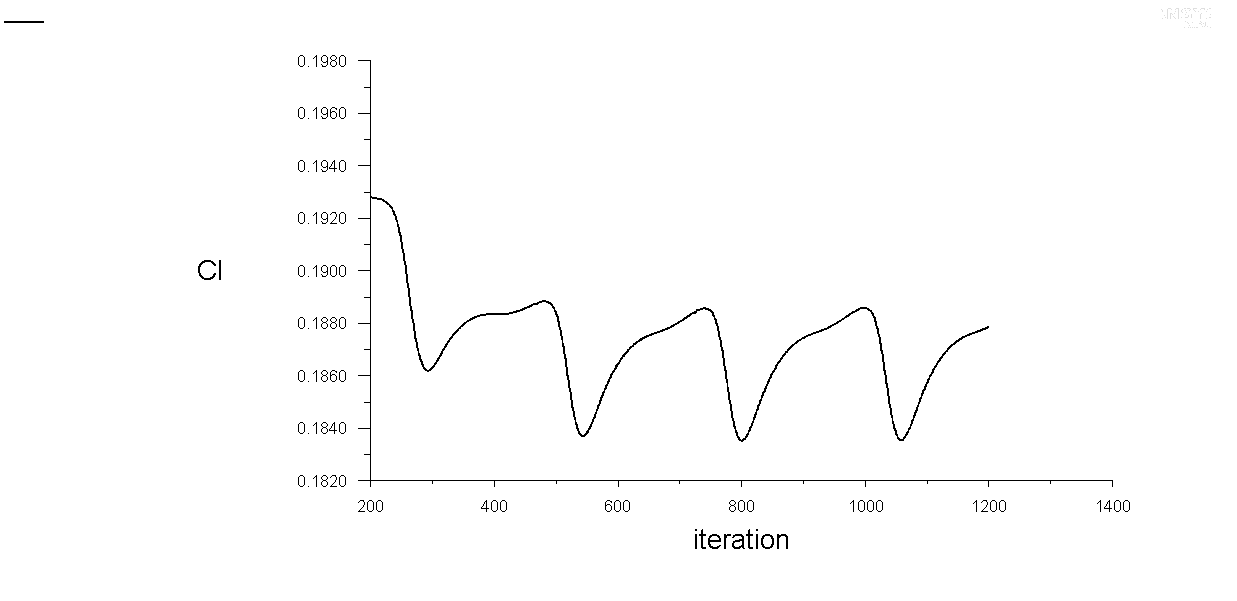
\includegraphics[width=\textwidth]{-2_deg/AoA_-2_cl.png}
    \caption{$C_l$ for AoA = -2$^\circ$}
    \label{fig:aoa_-2_cl}
  \end{subfigure}
  \hfill
  \begin{subfigure}[b]{0.5\textwidth}
    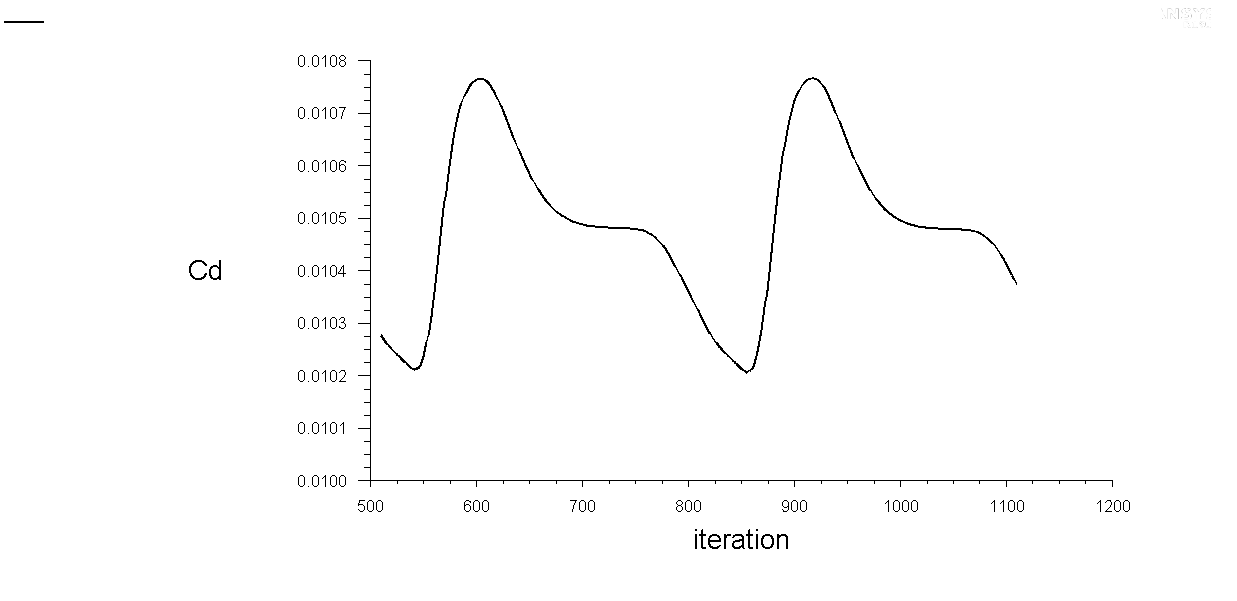
\includegraphics[width=\textwidth]{-2_deg/AoA_-2_cd.png}
    \caption{$C_d$ for AoA = -2$^\circ$}
    \label{fig:aoa_-2_cd}
  \end{subfigure}
  \begin{subfigure}[b]{0.5\textwidth}
    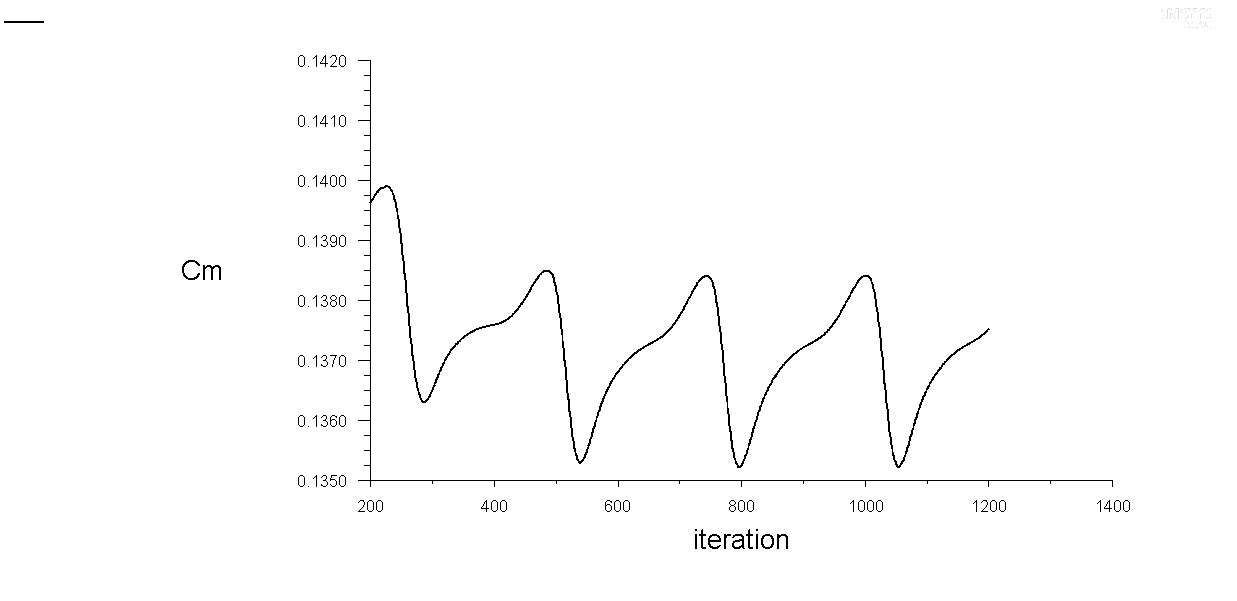
\includegraphics[width=\textwidth]{-2_deg/AoA_-2_cm.png}
    \caption{$C_m$ for AoA = -2$^\circ$}
    \label{fig:aoa_-2_cm}
  \end{subfigure}
  \begin{subfigure}[b]{0.5\textwidth}
    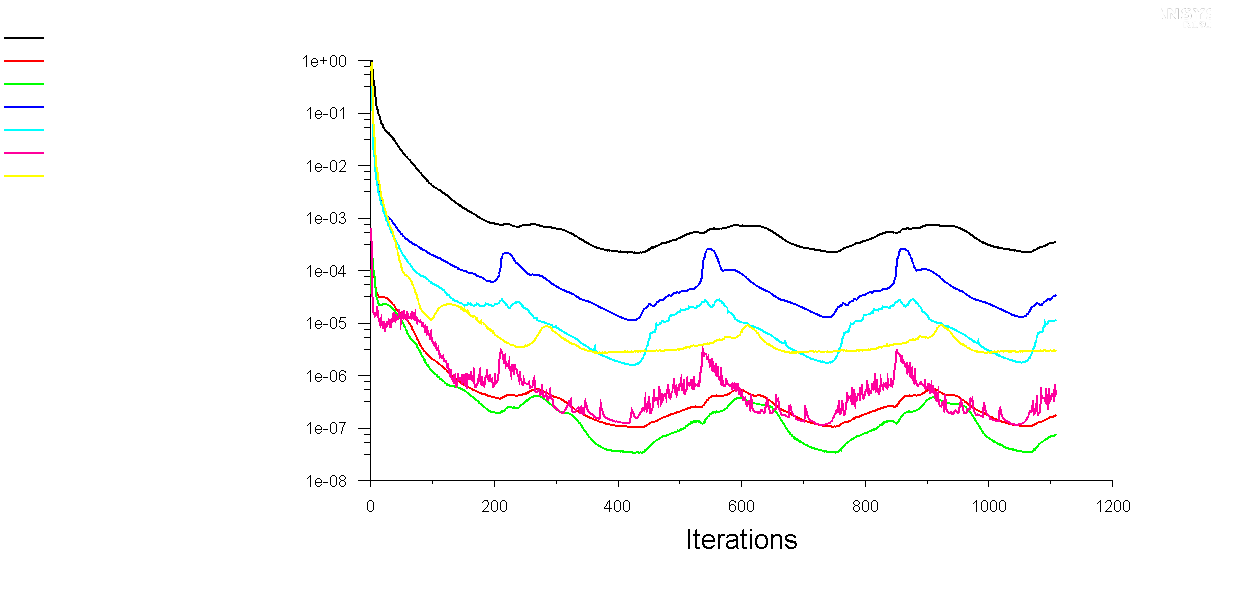
\includegraphics[width=\textwidth]{-2_deg/AoA_-2_resid.png}
    \caption{Residual plot for AoA = -2$^\circ$}
    \label{fig:aoa_-2_resid}
  \end{subfigure}
\end{figure}

% ************************ 0 degs ****************************
\subsection*{AoA = 0$^\circ$}

\begin{figure}[H]
  \begin{subfigure}[b]{0.5\textwidth}
    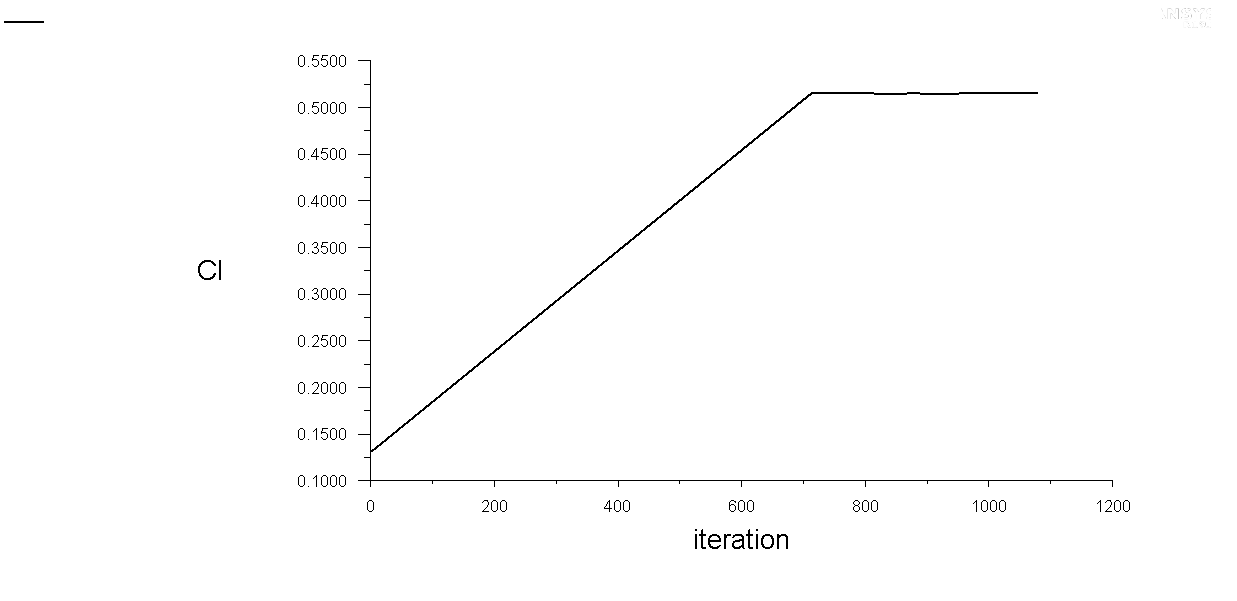
\includegraphics[width=\textwidth]{0_deg/AoA_0_cl.png}
    \caption{$C_l$ for AoA = 0$^\circ$}
    \label{fig:aoa_0_cl}
  \end{subfigure}
  \hfill
  \begin{subfigure}[b]{0.5\textwidth}
    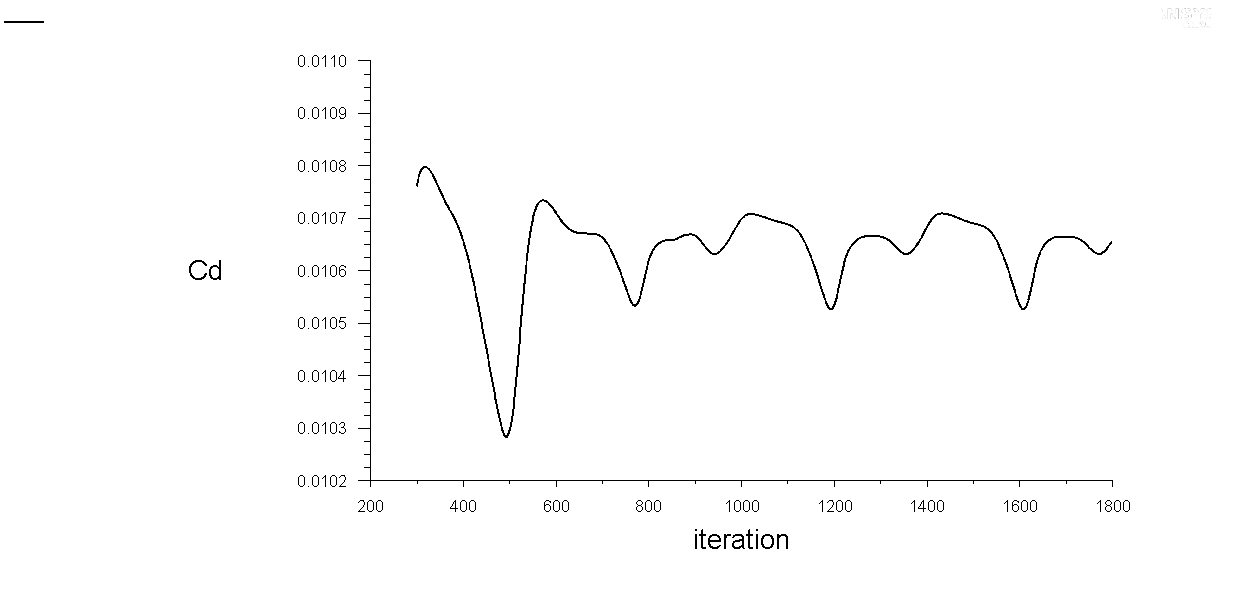
\includegraphics[width=\textwidth]{0_deg/AoA_0_cd.png}
    \caption{$C_d$ for AoA = 0$^\circ$}
    \label{fig:aoa_0_cd}
  \end{subfigure}
  \begin{subfigure}[b]{0.5\textwidth}
    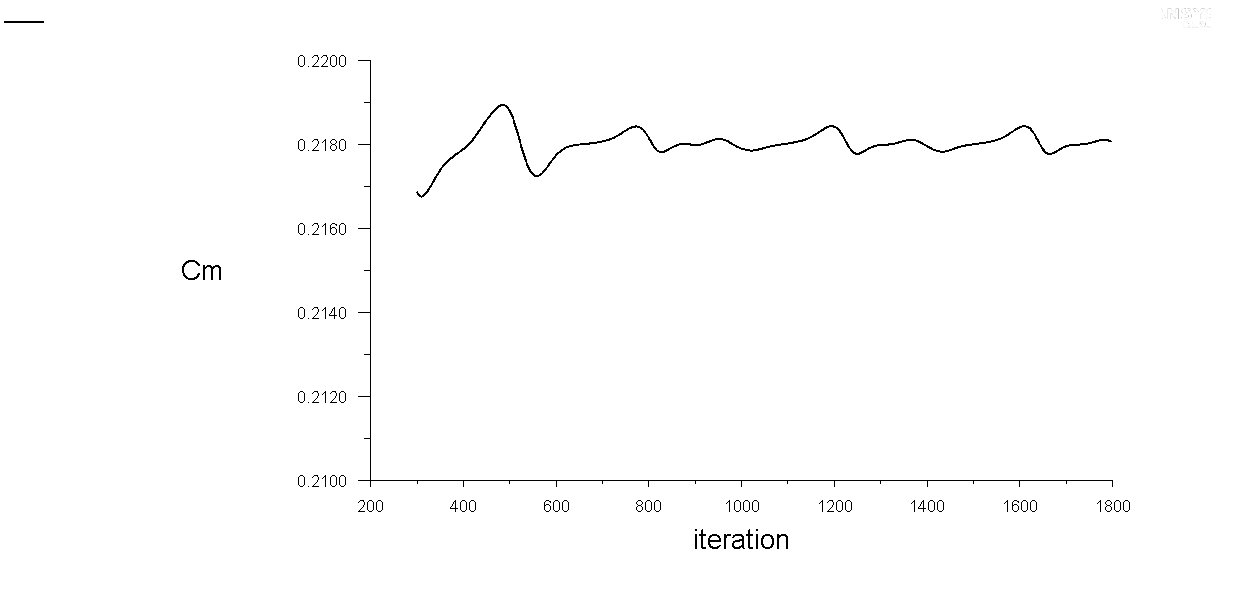
\includegraphics[width=\textwidth]{0_deg/AoA_0_cm.png}
    \caption{$C_m$ for AoA = 0$^\circ$}
    \label{fig:aoa_0_cm}
  \end{subfigure}
  \begin{subfigure}[b]{0.5\textwidth}
    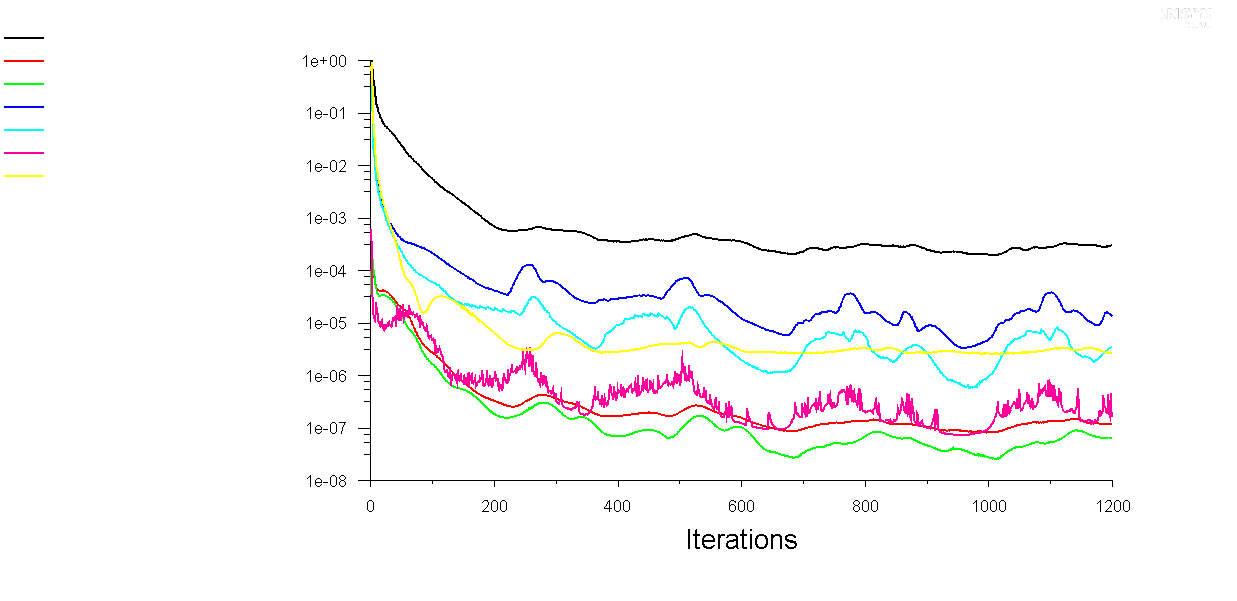
\includegraphics[width=\textwidth]{0_deg/AoA_0_resid.png}
    \caption{Residual plot for AoA = 0$^\circ$}
    \label{fig:aoa_0_resid}
  \end{subfigure}
\end{figure}

% ************************ 5 degs ****************************
\subsection*{AoA = 5$^\circ$}

\begin{figure}[H]
  \begin{subfigure}[b]{0.5\textwidth}
    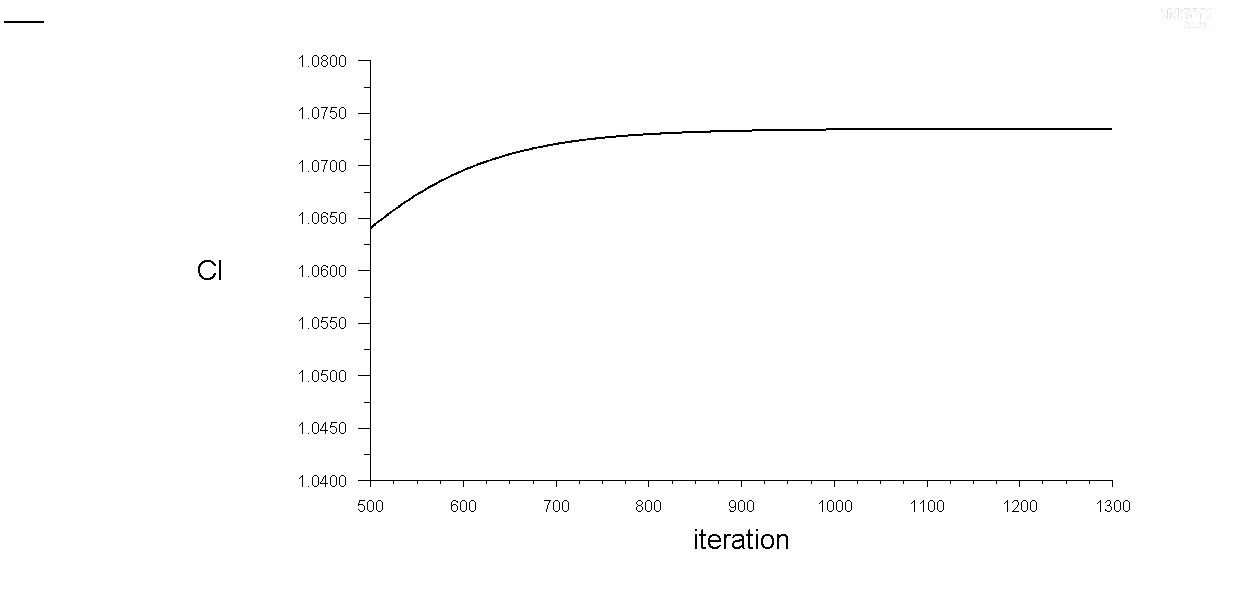
\includegraphics[width=\textwidth]{5_deg/AoA_5_cl.png}
    \caption{$C_l$ for AoA = 5$^\circ$}
    \label{fig:aoa_5_cl}
  \end{subfigure}
  \hfill
  \begin{subfigure}[b]{0.5\textwidth}
    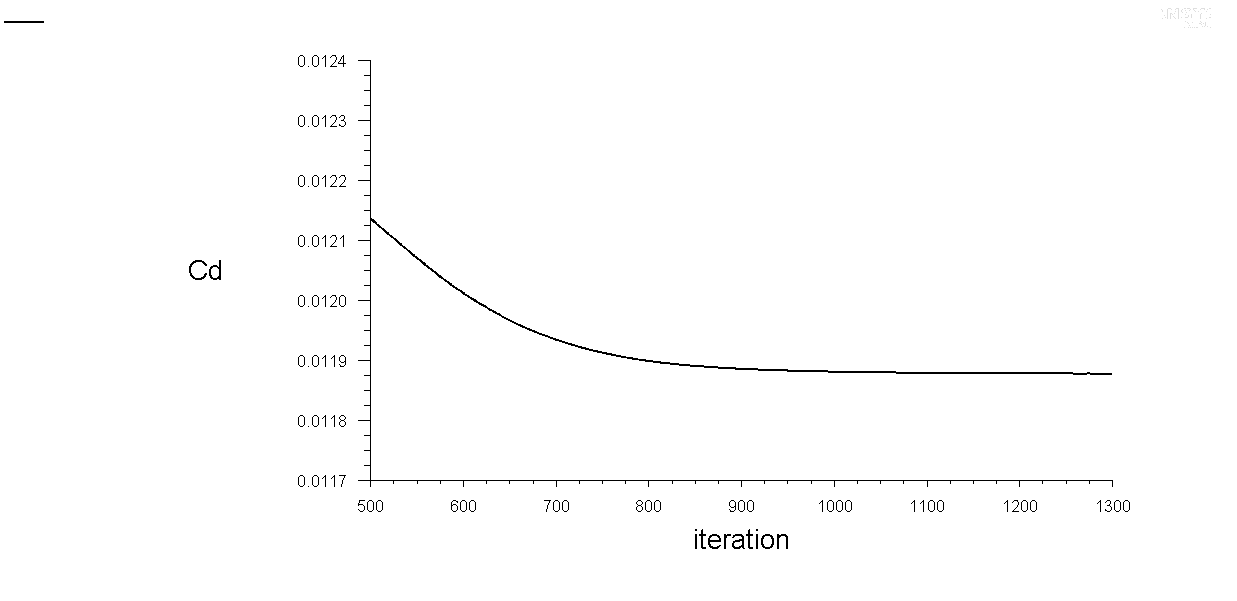
\includegraphics[width=\textwidth]{5_deg/AoA_5_cd.png}
    \caption{$C_d$ for AoA = 5$^\circ$}
    \label{fig:aoa_5_cd}
  \end{subfigure}
  \begin{subfigure}[b]{0.5\textwidth}
    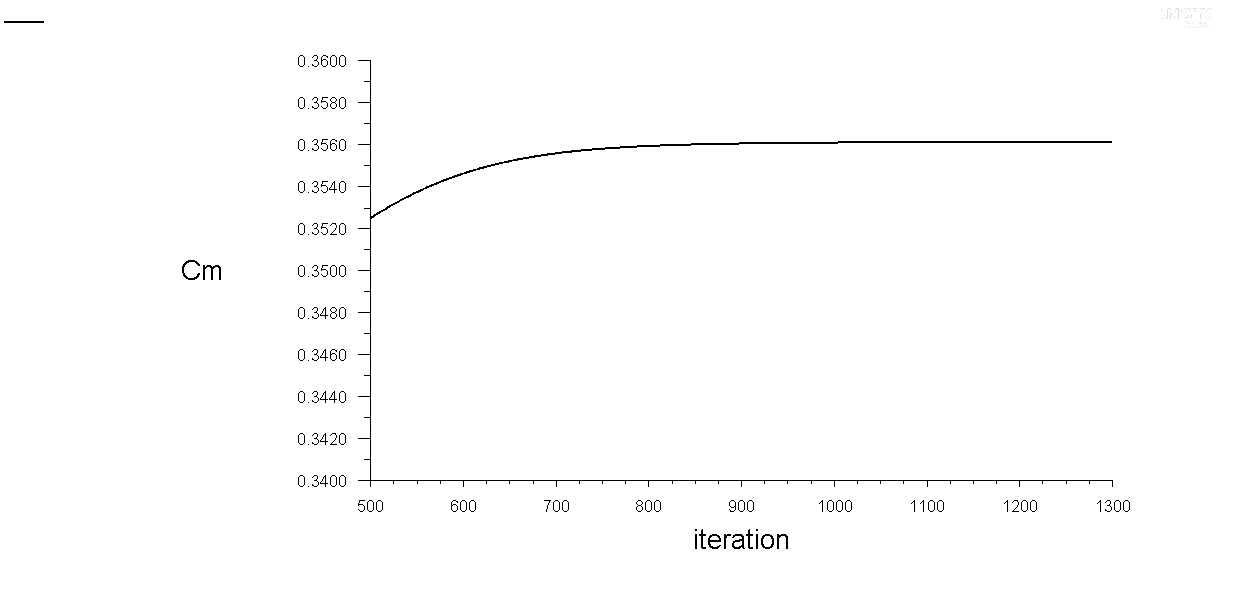
\includegraphics[width=\textwidth]{5_deg/AoA_5_cm.png}
    \caption{$C_m$ for AoA = 5$^\circ$}
    \label{fig:aoa_5_cm}
  \end{subfigure}
  \begin{subfigure}[b]{0.5\textwidth}
    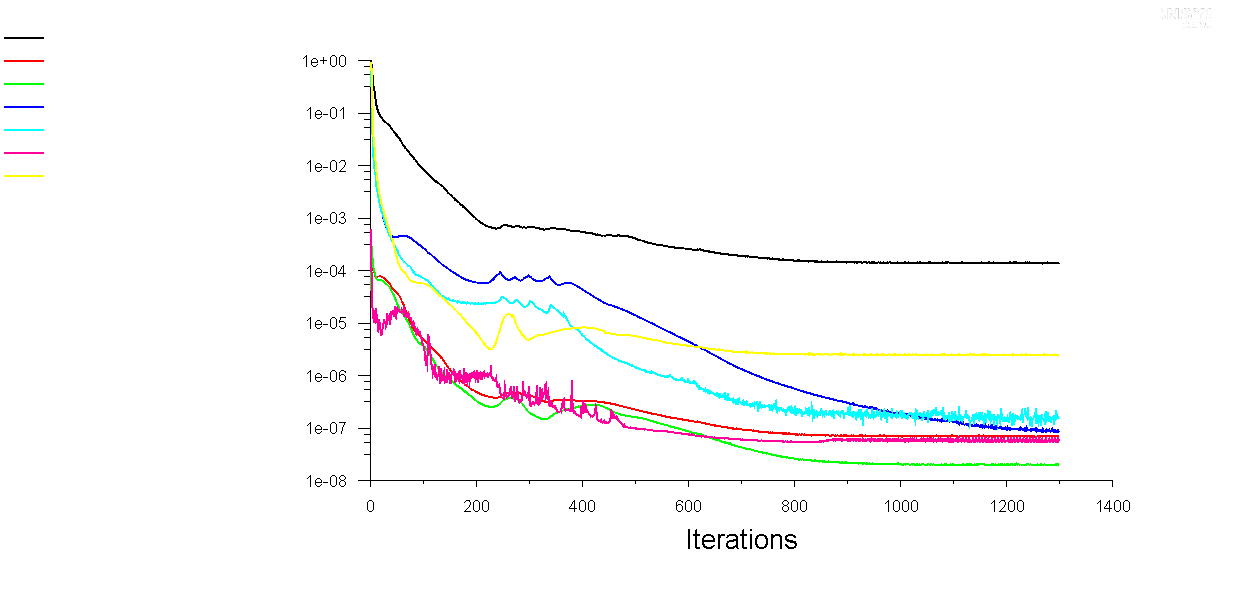
\includegraphics[width=\textwidth]{5_deg/AoA_5_resid.png}
    \caption{Residual plot for AoA = 5$^\circ$}
    \label{fig:aoa_5_resid}
  \end{subfigure}
\end{figure}

% ************************ 8.5 degs ****************************
\subsection*{AoA = 8.5$^\circ$}

\begin{figure}[H]
  \begin{subfigure}[b]{0.5\textwidth}
    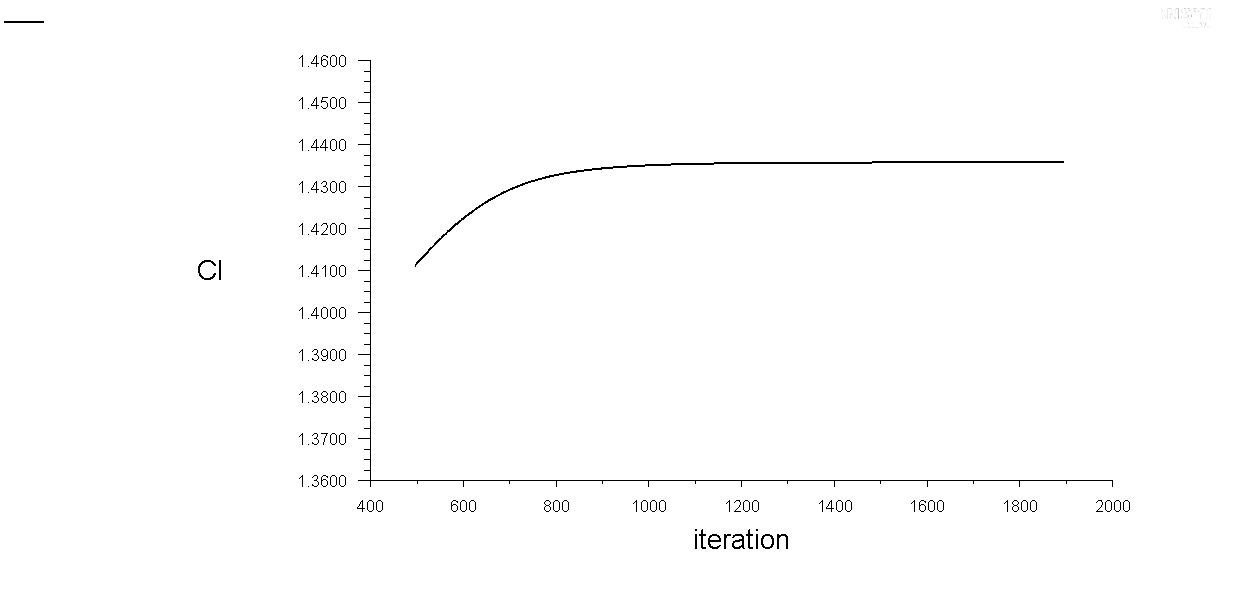
\includegraphics[width=\textwidth]{8.5_deg/AoA_8_5_cl.png}
    \caption{$C_l$ for AoA = 8.5$^\circ$}
    \label{fig:aoa_8.5_cl}
  \end{subfigure}
  \hfill
  \begin{subfigure}[b]{0.5\textwidth}
    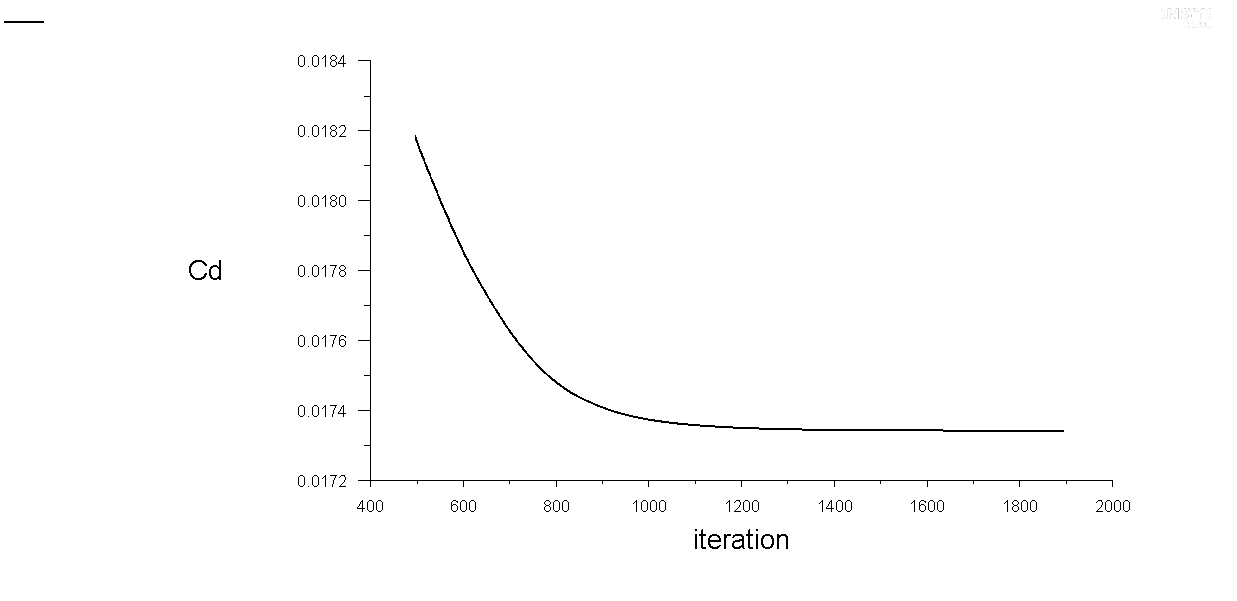
\includegraphics[width=\textwidth]{8.5_deg/AoA_8_5_cd.png}
    \caption{$C_d$ for AoA = 8.5$^\circ$}
    \label{fig:aoa_8.5_cd}
  \end{subfigure}
  \begin{subfigure}[b]{0.5\textwidth}
    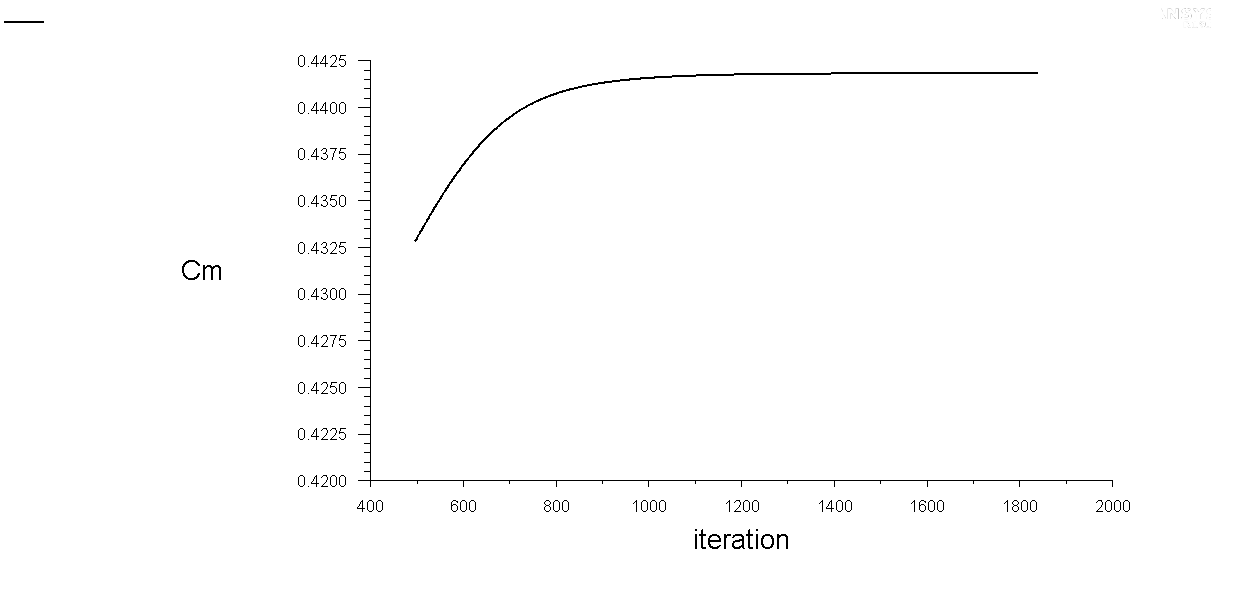
\includegraphics[width=\textwidth]{8.5_deg/AoA_8_5_cm.png}
    \caption{$C_m$ for AoA = 8.5$^\circ$}
    \label{fig:aoa_8.5_cm}
  \end{subfigure}
  \begin{subfigure}[b]{0.5\textwidth}
    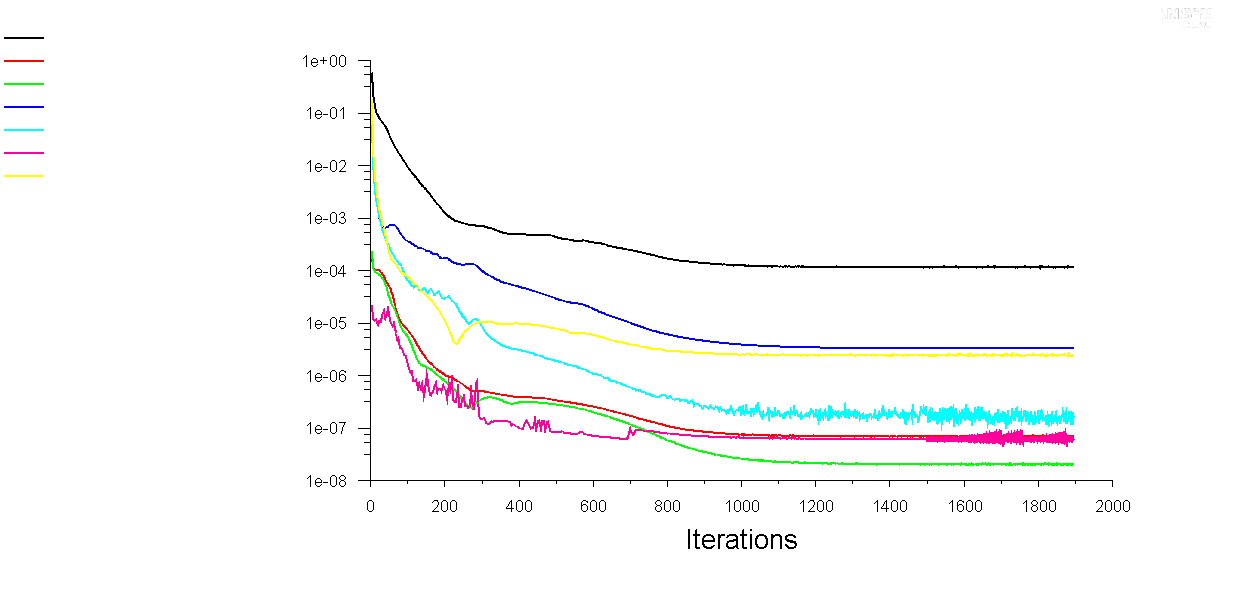
\includegraphics[width=\textwidth]{8.5_deg/AoA_8_5_resid.png}
    \caption{Residual plot for AoA = 8.5$^\circ$}
    \label{fig:aoa_8.5_resid}
  \end{subfigure}
\end{figure}

% ************************ 12 degs ****************************
\subsection*{AoA = 12$^\circ$}

\begin{figure}[H]
  \begin{subfigure}[b]{0.5\textwidth}
    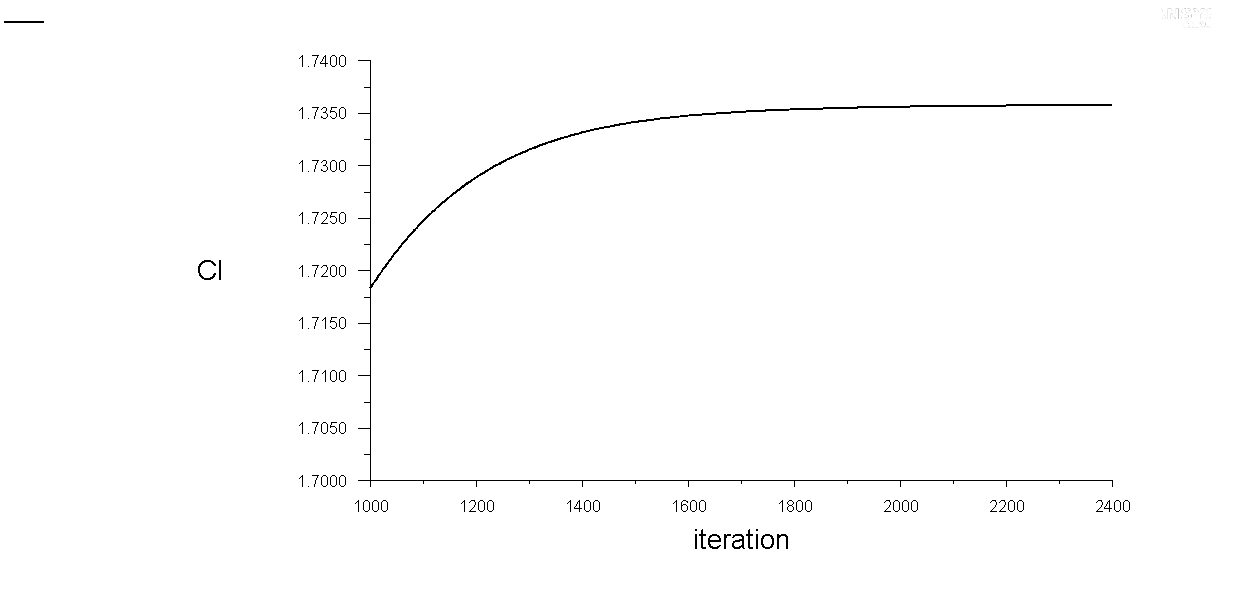
\includegraphics[width=\textwidth]{12_deg/AoA_12_cl.png}
    \caption{$C_l$ for AoA = 12$^\circ$}
    \label{fig:aoa_12_cl}
  \end{subfigure}
  \hfill
  \begin{subfigure}[b]{0.5\textwidth}
    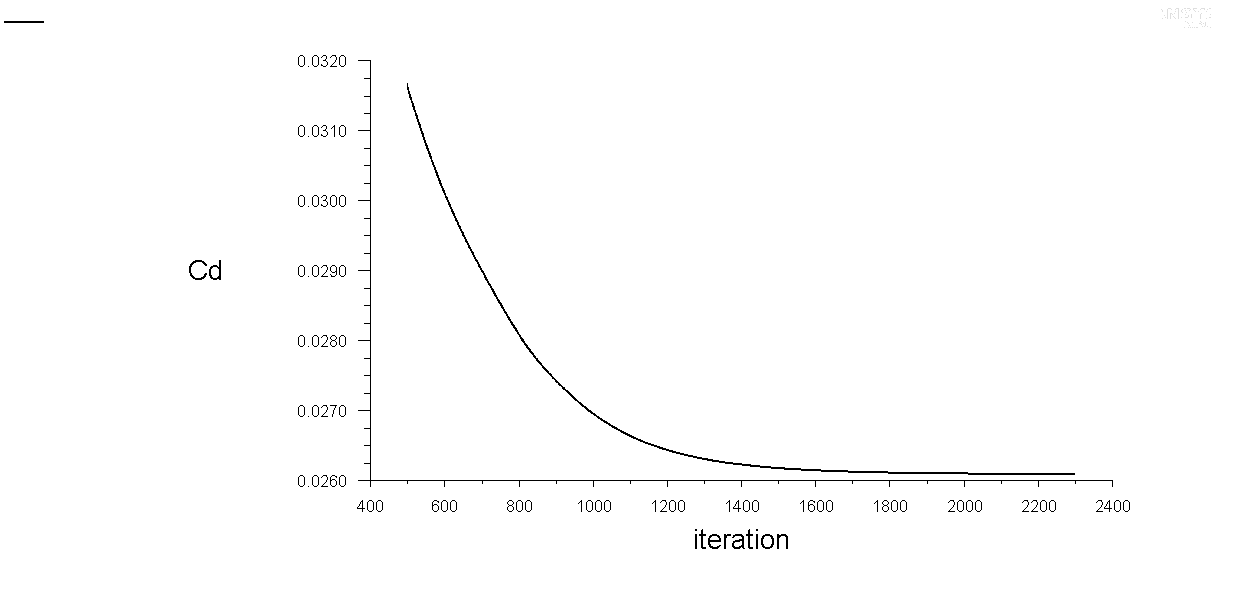
\includegraphics[width=\textwidth]{12_deg/AoA_12_cd.png}
    \caption{$C_d$ for AoA = 12$^\circ$}
    \label{fig:aoa_12_cd}
  \end{subfigure}
  \begin{subfigure}[b]{0.5\textwidth}
    \includegraphics[width=\textwidth]{12_deg/AoA_12_cm.png}
    \caption{$C_m$ for AoA = 12$^\circ$}
    \label{fig:aoa_12_cm}
  \end{subfigure}
  \begin{subfigure}[b]{0.5\textwidth}
    \includegraphics[width=\textwidth]{12_deg/AoA_12_resid.png}
    \caption{Residual plot for AoA = 12$^\circ$}
    \label{fig:aoa_12_resid}
  \end{subfigure}
\end{figure}

% ************************ 14.5 degs ****************************
\subsection*{AoA = 14.5$^\circ$}

\begin{figure}[H]
  \begin{subfigure}[b]{0.5\textwidth}
    \includegraphics[width=\textwidth]{14.5_deg/AoA_14_5_cl.png}
    \caption{$C_l$ for AoA = 14.5$^\circ$}
    \label{fig:aoa_14.5_cl}
  \end{subfigure}
  \hfill
  \begin{subfigure}[b]{0.5\textwidth}
    \includegraphics[width=\textwidth]{14.5_deg/AoA_14_5_cd.png}
    \caption{$C_d$ for AoA = 14.5$^\circ$}
    \label{fig:aoa_14.5_cd}
  \end{subfigure}
  \begin{subfigure}[b]{0.5\textwidth}
    \includegraphics[width=\textwidth]{14.5_deg/AoA_14_5_cm.png}
    \caption{$C_m$ for AoA = 14.5$^\circ$}
    \label{fig:aoa_14.5_cm}
  \end{subfigure}
  \begin{subfigure}[b]{0.5\textwidth}
    \includegraphics[width=\textwidth]{14.5_deg/AoA_14_5_resid.png}
    \caption{Residual plot for AoA = 14.5$^\circ$}
    \label{fig:aoa_14.5_resid}
  \end{subfigure}
\end{figure}

% ************************ 17 degs ****************************
\subsection*{AoA = 17$^\circ$}

\begin{figure}[H]
  \begin{subfigure}[b]{0.5\textwidth}
    \includegraphics[width=\textwidth]{17_deg/AoA_17_cl.png}
    \caption{$C_l$ for AoA = 17$^\circ$}
    \label{fig:aoa_17_cl}
  \end{subfigure}
  \hfill
  \begin{subfigure}[b]{0.5\textwidth}
    \includegraphics[width=\textwidth]{17_deg/AoA_17_cd.png}
    \caption{$C_d$ for AoA = 17$^\circ$}
    \label{fig:aoa_17_cd}
  \end{subfigure}
  \begin{subfigure}[b]{0.5\textwidth}
    \includegraphics[width=\textwidth]{17_deg/AoA_17_cm.png}
    \caption{$C_m$ for AoA = 17$^\circ$}
    \label{fig:aoa_17_cm}
  \end{subfigure}
  \begin{subfigure}[b]{0.5\textwidth}
    \includegraphics[width=\textwidth]{17_deg/AoA_17_resid.png}
    \caption{Residual plot for AoA = 17$^\circ$}
    \label{fig:aoa_17_resid}
  \end{subfigure}
\end{figure}

% ************************ 19.5 degs ****************************
\subsection*{AoA = 19.5$^\circ$}

\begin{figure}[H]
  \begin{subfigure}[b]{0.5\textwidth}
    \includegraphics[width=\textwidth]{19.5_deg/AoA_19_5_cl.png}
    \caption{$C_l$ for AoA = 19.5$^\circ$}
    \label{fig:aoa_19.5_cl}
  \end{subfigure}
  \hfill
  \begin{subfigure}[b]{0.5\textwidth}
    \includegraphics[width=\textwidth]{19.5_deg/AoA_19_5_cd.png}
    \caption{$C_d$ for AoA = 19.5$^\circ$}
    \label{fig:aoa_19.5_cd}
  \end{subfigure}
  \begin{subfigure}[b]{0.5\textwidth}
    \includegraphics[width=\textwidth]{19.5_deg/AoA_19_5_cm.png}
    \caption{$C_m$ for AoA = 19.5$^\circ$}
    \label{fig:aoa_19.5_cm}
  \end{subfigure}
  \begin{subfigure}[b]{0.5\textwidth}
    \includegraphics[width=\textwidth]{19.5_deg/AoA_19_5_resid.png}
    \caption{Residual plot for AoA = 19.5$^\circ$}
    \label{fig:aoa_19.5_resid}
  \end{subfigure}
\end{figure}

% ************************ 22 degs ****************************
\subsection*{AoA = 22$^\circ$}

\begin{figure}[H]
  \begin{subfigure}[b]{0.5\textwidth}
    \includegraphics[width=\textwidth]{22_deg/AoA_22_cl.png}
    \caption{$C_l$ for AoA = 22$^\circ$}
    \label{fig:aoa_22_cl}
  \end{subfigure}
  \hfill
  \begin{subfigure}[b]{0.5\textwidth}
    \includegraphics[width=\textwidth]{22_deg/AoA_22_cd.png}
    \caption{$C_d$ for AoA = 22$^\circ$}
    \label{fig:aoa_22_cd}
  \end{subfigure}
  \begin{subfigure}[b]{0.5\textwidth}
    \includegraphics[width=\textwidth]{22_deg/AoA_22_cm.png}
    \caption{$C_m$ for AoA = 22$^\circ$}
    \label{fig:aoa_22_cm}
  \end{subfigure}
  \begin{subfigure}[b]{0.5\textwidth}
    \includegraphics[width=\textwidth]{22_deg/AoA_22_resid.png}
    \caption{Residual plot for AoA = 22$^\circ$}
    \label{fig:aoa_22_resid}
  \end{subfigure}
\end{figure}



%\begin{figure}[h!]
%\centering
%\includegraphics[scale=1.7]{universe}
%\caption{The Universe}
%\label{fig:universe}
%\end{figure}

%\section{Conclusion}
%``I always thought something was fundamentally wrong with the universe'' \citep{adams1995hitchhiker}

\bibliographystyle{plain}
\bibliography{references}
\end{document}
